%%%%%%%%%%%%%%%%%%%%%%%%%%%%%%%%%%%%%%%%%%%%%%%%%%%%%%%%%%%%%%
\fe{\section{Calcul mécanique}}{\section{Mechanical Calculation}}
\label{mecanique}
%%%%%%%%%%%%%%%%%%%%%%%%%%%%%%%%%%%%%%%%%%%%%%%%%%%%%%%%%%%%%%

\fe{\subsection{Mécanique linéaire}}{\subsection{Linear Mechanics}}
\begin{frame}{\fe{Mécanique}{Mechanics}}{\fe{Rappels}{Reminders}}
  \begin{itemize}
    \item \fe{Équation d'équilibre statique}{Static equilibrium equation}
    \begin{block}{\fe{Forme locale}{Local form}}
      \begin{equation*}
        \tx{div}(\tod{\sigma})+\tou{f}=\tou{0}\quad\fe{\tx{sur }V}{\tx{on }V}
      \end{equation*}
    \end{block}~
    \item \fe{Conditions aux limites}{Boundary conditions}\\
    \footnotesize
%    \setlength\tabcolsep{1.5pt}
    \fe{\begin{tabular}{lrll}
          Déplacements imposés & $\tou{u}$              & $=\tou{u}_{\tx{imp}}$ & sur $\partial V_u$\\
          Efforts imposés      & $\tod{\sigma}.\tou{n}$ & $=\tou{t}_{\tx{imp}}$ & sur $\partial V_t$\\
        \end{tabular}}
       {\begin{tabular}{lrll}
          Imposed displacements & $\tou{u}$              & $=\tou{u}_{\tx{imp}}$ & on $\partial V_u$\\
          Imposed forces        & $\tod{\sigma}.\tou{n}$ & $=\tou{t}_{\tx{imp}}$ & on $\partial V_t$\\
        \end{tabular}}
    \normalsize
    \item \fe{Avec}{With}
    \begin{itemize}
      \item[] $\tou{u}$ \fe{vecteur déplacement}{displacement vector}
      \item[] $\tod{\sigma}$ \fe{tenseur des contraintes}{stress tensor}
      \item[] $\tou{f}$ \fe{vecteur des forces volumiques}{volumic forces vector}
      \item[] $\tou{n}$ \fe{vecteur normal à la surface}{normal vector to a surface}
    \end{itemize}
    \normalsize
  \end{itemize}
\end{frame}

\begin{frame}{\fe{Mécanique}{Mechanics}}{\fe{Rappels}{Reminders}}
  \small
  \begin{itemize}
    \item \fe{Éléments finis :}{Finite elements:} $\tou{u}(x)=[N(x)]\{U\}$
    \begin{block}{\fe{Formulation faible et discrétisée de l'équilibre :}
                     {Weak and discrete formulation of equilibrium:}}
      \begin{equation*}
        \int_{V}[B]^T\{\sigma\}dV=\{F\}
      \end{equation*}
    \end{block}~\\
    \footnotesize
    \begin{center}
      $\underbrace{\int_{V}[B]^T\{\sigma\}dV}_{[B]\{\sigma\}}=\underbrace{\int_{\partial V_t}[N]^T\{t\}_{\tx{imp}}dS}_{\{F\}_{\tx{s}}}+\underbrace{\int_{\partial V_u}[N]^T\{\sigma .n\}dS}_{\{F\}_{\tx{reac}}}+\underbrace{\int_{V}[N]^T\{f\}_{\tx{s}}dV}_{\{F\}_{\tx{v}}}$
    \end{center}
    \scriptsize
    \fe{Vecteurs de forces nodales équivalentes aux :}{Equivalent nodal forces vector to:}
    \scriptsize
    \begin{tabular}{ll}
      $\{F\}_{\tx{s}}$    & \fe{densité surfacique d'efforts imposés $\tou{t}_{\tx{imp}}$}
                               {imposed surface forces $\tou{t}_{\tx{imp}}$}\\
      $\{F\}_{\tx{reac}}$ & \fe{densité surfacique de réaction aux déplacements imposés $\tou{u}_{\tx{imp}}$}
                               {surface reactions to imposed displacements $\tou{u}_{\tx{imp}}$}\\
      $\{F\}_{\tx{v}}$    & \fe{densité volumique d'efforts imposés $\tou{f}_{\tx{imp}}$}{imposed volume forces $\tou{f}_{\tx{imp}}$}\\
      $[B]\{\sigma\}$     & \fe{densité volumique d'efforts intérieurs}{internal volume forces}
    \end{tabular}\\
    \fe{Matrices :}{Matrices:}\\
    \begin{tabular}{ll}
      $[N]$ & \fe{matrice des fonctions de forme}{matrix of shape functions}\\
      $[B]$ & \fe{matrice des dérivées des fonctions de forme}{matrix of derivative of shape functions}
     \end{tabular}
  \end{itemize}
  \normalsize
\end{frame}

\begin{frame}{\fe{Mécanique}{Mechanics}}{\fe{Rappels}{Reminders}}
  \begin{itemize}
    \item \fe{Hypothèse des petites déformations :}{Infinitesimal strains hypothesis:} $\{\varepsilon\}=[B]\{U\}$
    \item \fe{Élasticité linéaire :}{Linear elasticity:} $\{\sigma\}=[C]\{\varepsilon\}$
    \begin{block}{\fe{Formulation faible et discrétisée de l'équilibre :}
                     {Weak and discrete formulation of equilibrium:}}
      \begin{equation*}
        \underbrace{\int_{V}[B]^T[C][B]dV}_{[K]}\{U\}=\{F\}
      \end{equation*}
    \end{block}~\\
    \fe{Matrices :}{Matrices:}\\
    \begin{tabular}{ll}
      $[C]$ & \fe{matrice de Hooke}{Hooke matrix}\\
      $[K]$ & \fe{matrice de rigidité}{stifness matrix}
    \end{tabular}
  \end{itemize}
\end{frame}

\begin{frame}{\fe{6 Problème étudié}{6 Problem description}}
  \begin{itemize}
    \item \fe{Élasticité linéaire}{Linear elasticity}
    \begin{center}
    \footnotesize
    \begin{tikzpicture}
      \node[anchor=south west,inner sep=0] (image) at (0,0)
      {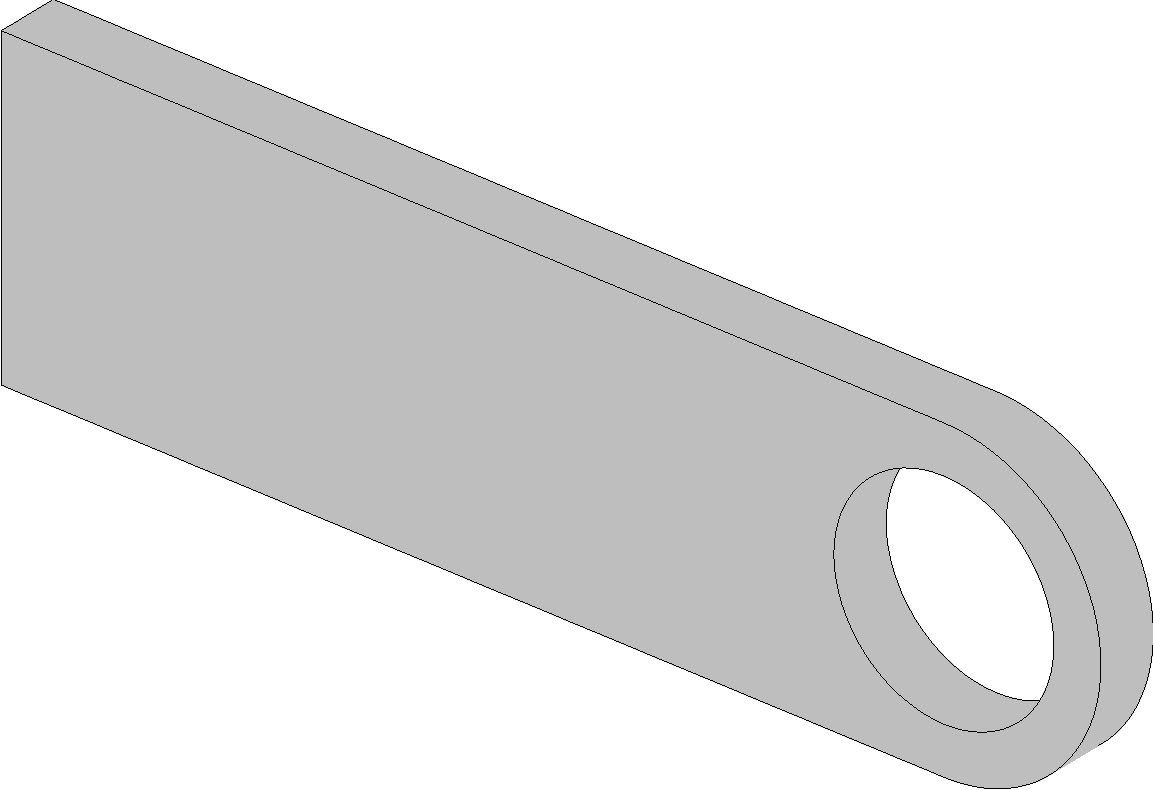
\includegraphics[width=4cm]{images/exo/1.2_geometrie}};
      \begin{scope}[x={(image.south east)},y={(image.north west)}]
        \draw (1,0.9) node[anchor=west] {$E$~=~200~GPa};
        \draw (1,0.7) node[anchor=west] {$\nu$~=~0.3};
        \draw (1,0.5) node[anchor=west] {$\alpha$~=~10$^{-5}$~K$^{-1}$};
      \end{scope}
    \end{tikzpicture}
    \normalsize
    \end{center}
    \begin{columns}
      \begin{column}{.4\textwidth}
        \item \fe{Déplacements imposés}{Imposed displacements}
        \footnotesize
        \begin{tikzpicture}
          \node[anchor=south west,inner sep=0] (image) at (0,0)
          {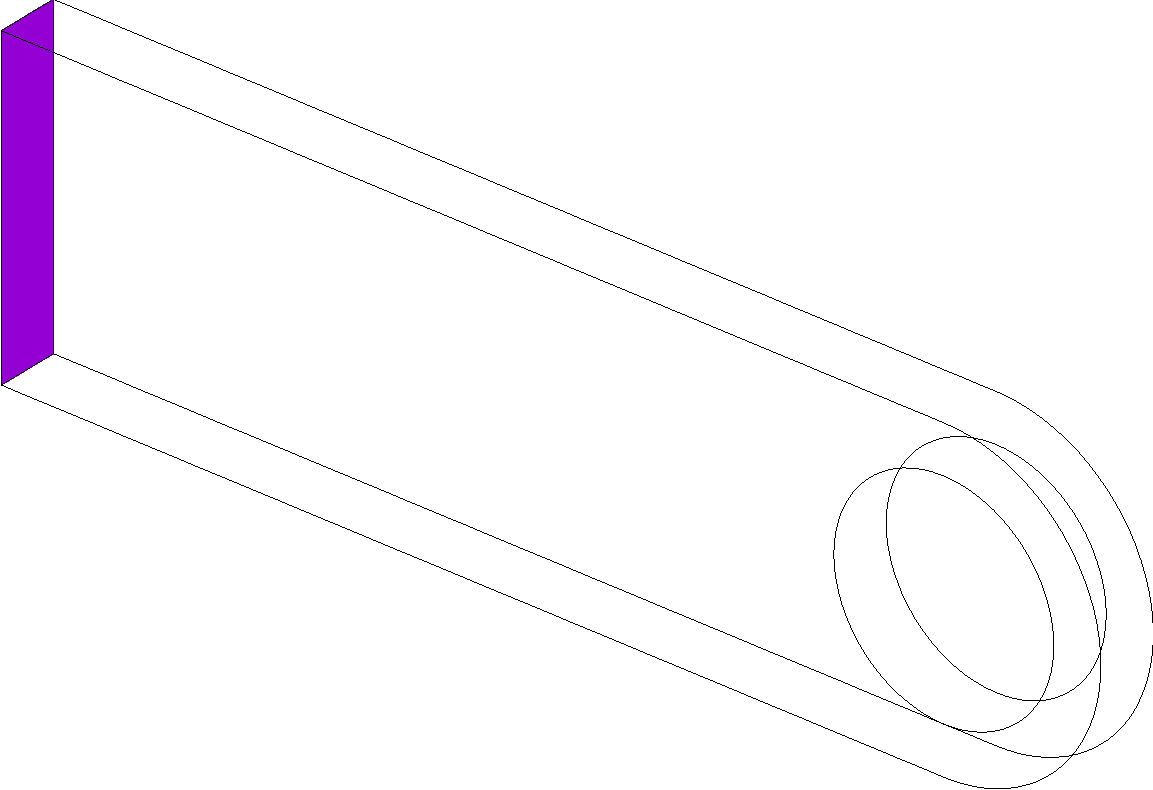
\includegraphics[width=3.5cm]{images/exo/6_cl_deplacement}};
          \begin{scope}[x={(image.south east)},y={(image.north west)},color=violet]
            \draw (0.06,0.7) node[anchor=north west] {$u_x=u_y=u_z$~=~0~m};
          \end{scope}
        \end{tikzpicture}
        \normalsize
      \end{column}
      \begin{column}{.4\textwidth}
        \item \fe{Forces imposées}{Imposed forces}
        \footnotesize
        \begin{tikzpicture}
          \node[anchor=south west,inner sep=0] (image) at (0,0)
          {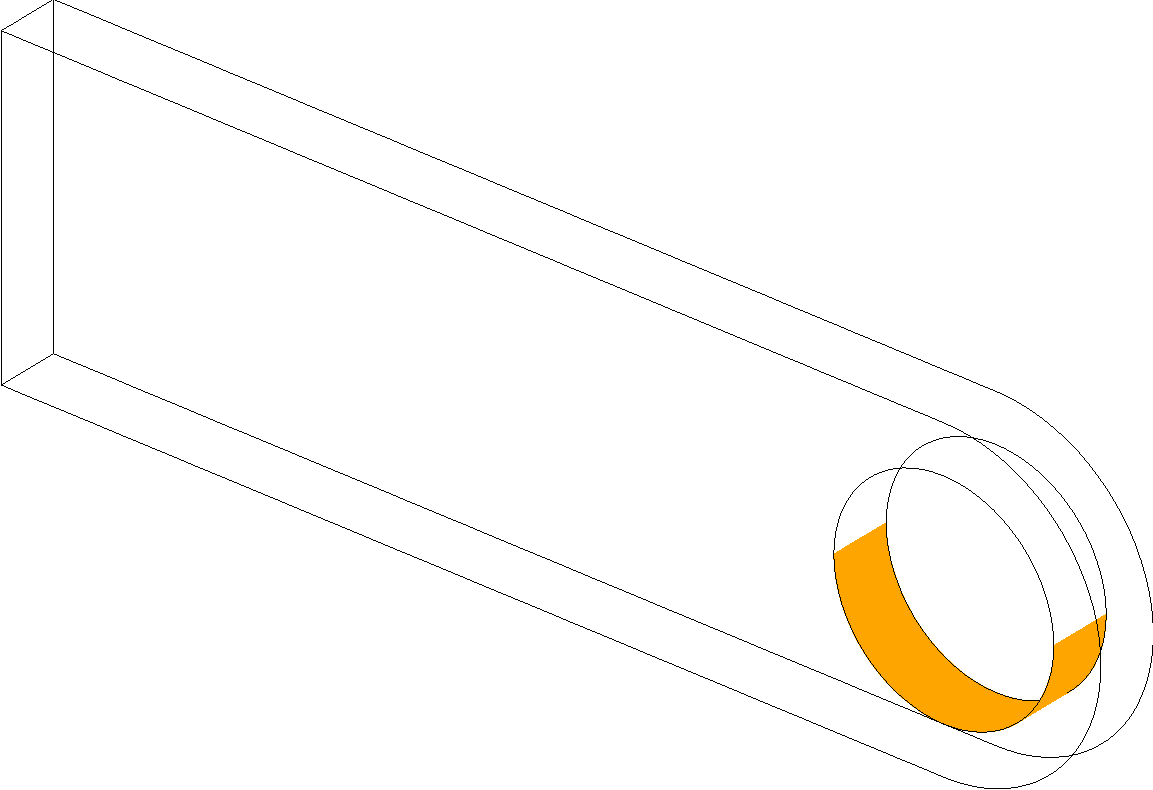
\includegraphics[width=3.5cm]{images/exo/6_cl_force}};
          \begin{scope}[x={(image.south east)},y={(image.north west)},color=orange]
            \draw (0.8,0.75) node[anchor=north west] {\fe{masse suspendue}{hanging mass}};
            \draw (0.9,0.6) node[anchor=north west] {$m$~=~2500~kg};
          \end{scope}
        \end{tikzpicture}
        \normalsize
      \end{column}
    \end{columns}
  \end{itemize}
\end{frame}

\begin{frame}{\fe{6 Mécanique linéaire}{6 Linear mechanics}}
             {\fe{Élasticité}{Elasticity}}
  \begin{itemize}
    \item \fe{Objectif : calcul mécanique linéaire\\
              en déplacements et forces imposées}
            {Objective: linear mechanical calculation\\
             with fixed displacements and forces}
    \begin{center}
      $[K]\{U\}=\{F\}$ \qquad $\Rightarrow$ \fe{Système linéaire}{Linear system}
    \end{center}
    \item \fe{Méthode :}{Method:}\\
    \begin{tabular}{ll}
      \fe{calcul de la matrice de rigidité}{stiffness matrix calculation} & $[K]$\\
      \fe{calcul des chargement nodaux équivalents}{fixed nodal forces loads calculation} & $\{F\}$\\
      \fe{résolution avec \kwr{RESO}}{sovling with \kwr{RESO}} & $\{U\}=[K]^{-1}\{F\}$
    \end{tabular}
  \end{itemize}
\end{frame}



\begin{frame}{\fe{6 Mécanique linéaire}{6 Linear mechanics}}
             {\fe{Élasticité}{Elasticity}}
  \begin{itemize}
    \item \fe{Restitution des objets (maillage, paramètres, …)}
             {Input data from previous computation (mesh, parameters, …)}
    \lstinputlisting[language=gibiane, firstline=28, lastline=29]{dgibi/formation_debutant_3_mecanique.dgibi}
    \item \fe{Nouveaux paramètres}{New parameters}
    \lstinputlisting[language=gibiane, firstline=42, lastline=45]{dgibi/formation_debutant_3_mecanique.dgibi}
    \lstinputlisting[language=gibiane, firstline=48, lastline=50]{dgibi/formation_debutant_3_mecanique.dgibi}
  \end{itemize}
\end{frame}

\begin{frame}{\fe{6 Mécanique linéaire}{6 Linear mechanics}}
             {\fe{Élasticité}{Elasticity}}
  \begin{itemize}
    \item \fe{Formulation mathématique (élasticité)}{Mathematical formulation (elasticity)}
    \lstinputlisting[language=gibiane, firstline=68, lastline=71]{dgibi/formation_debutant_3_mecanique.dgibi}
    \item<2->\fe{Matrice de rigidité}{Stifness matrix}
    \onslide<2->{
      \lstinputlisting[language=gibiane, firstline=73, lastline=74]{dgibi/formation_debutant_3_mecanique.dgibi}
      \begin{flushright}
        \footnotesize
        $[K]=\int_V[B]^T[C][B]dV$
        \normalsize
      \end{flushright}}
    \item<3->\fe{Conditions aux limites}{Boundary conditions}
    \onslide<3->{
      \lstinputlisting[language=gibiane, firstline=76, lastline=77]{dgibi/formation_debutant_3_mecanique.dgibi}}
  \end{itemize}
\end{frame}

\begin{frame}{\fe{6 Mécanique linéaire}{6 Linear mechanics}}
             {\fe{Élasticité}{Elasticity}}
  \begin{itemize}
    \item \fe{Comment représenter le chargement ?}{How to represent the load?}
    \only<1>{\vspace{7cm}}
    \only<2-4>{
    \item \fe{1) Avec une \g{\tou{force ponctuelle}}}{1) With a \g{\tou{single point force}}}\\
    \begin{textblock*}{5cm}(8.7cm,-2.4cm)
      \begin{tikzpicture}
        \scriptsize
        \node[anchor=south west,inner sep=0] (image) at (0,0)
        {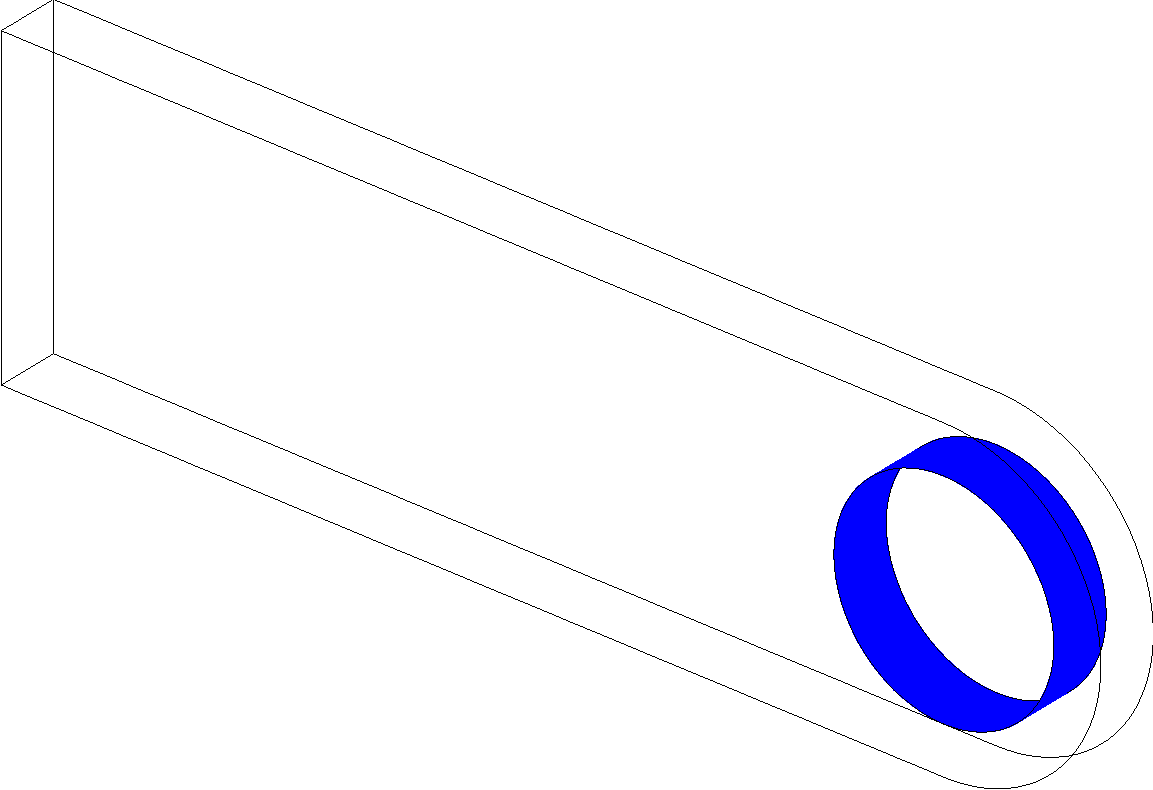
\includegraphics[width=3.5cm]{images/exo/2.1_cl_temperature}};
        \begin{scope}[x={(image.south east)},y={(image.north west)}]
          \draw (0.85,0.5) node {\kwb{sint}};
          \filldraw[black] (0.85,0.1) circle (1pt) node[anchor=north]{\kw{ptmass}};
        \end{scope}
      \end{tikzpicture}
    \end{textblock*}
    \avous{\fe{Récupérer le "centre" de la surface (voir : POIN 'PROC')}
              {Get the "center" of the surface (see: POIN 'PROC')}}\\
    \avous{\fe{Appliquer une force ponctuelle (voir : FORC)}
              {Apply a single point force (see: FORC)}}
    \onslide<3-4>{
      \lstinputlisting[language=gibiane, firstline=88, lastline=89]{dgibi/formation_debutant_3_mecanique.dgibi}}
    \onslide<4>{
      \lstinputlisting[language=gibiane, firstline=90, lastline=90]{dgibi/formation_debutant_3_mecanique.dgibi}
      \lstinputlisting[language=gibiane, firstline=95, lastline=95]{dgibi/formation_debutant_3_mecanique.dgibi}
      \begin{textblock*}{5cm}(7.8cm,-0.5cm)
        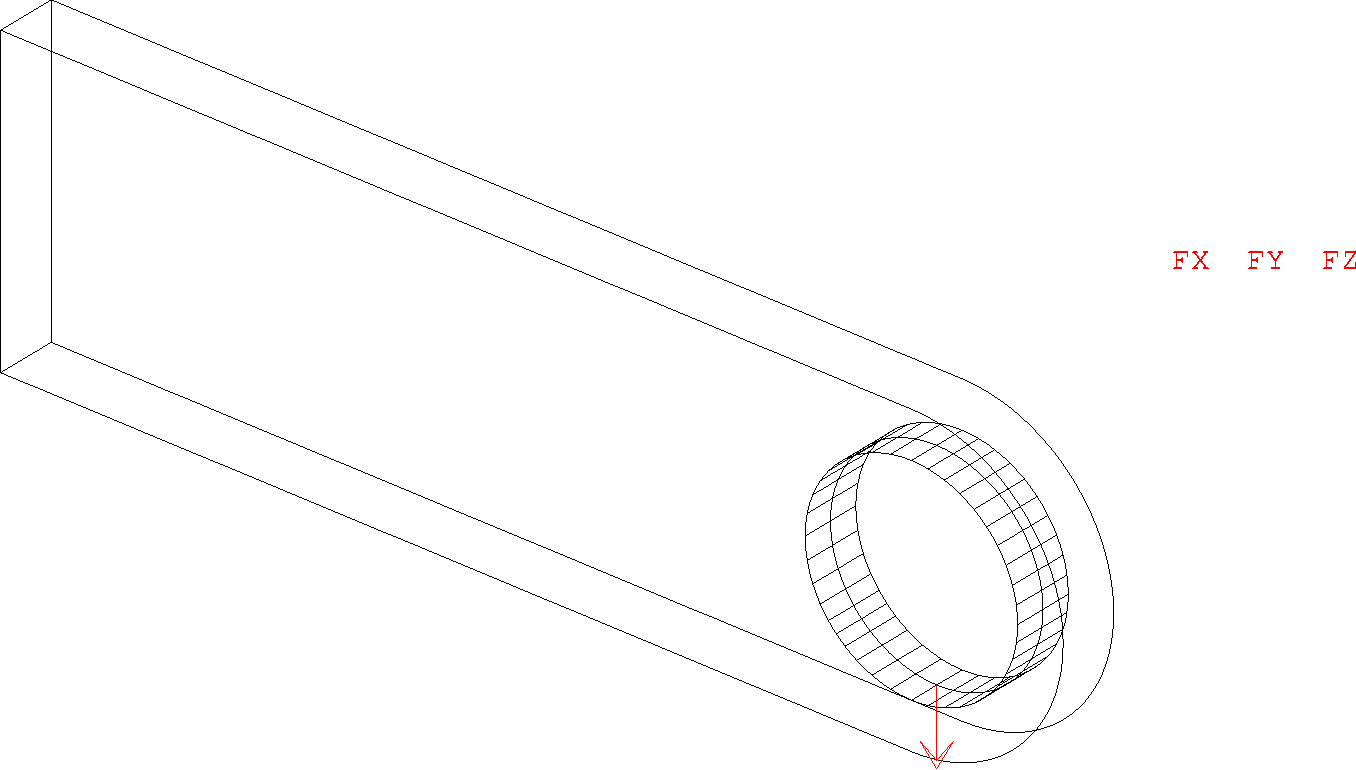
\includegraphics[width=4.5cm]{images/exo/6_forces.1}
      \end{textblock*}}
    \vspace{5cm}
    }
    \only<5-7>{
    \item \fe{2) Avec une \g{\tou{pression}}}{2) With a \g{\tou{pressure}}}\\
    \begin{textblock*}{5cm}(8.7cm,-2.4cm)
      \begin{tikzpicture}
        \scriptsize
        \node[anchor=south west,inner sep=0] (image) at (0,0)
        {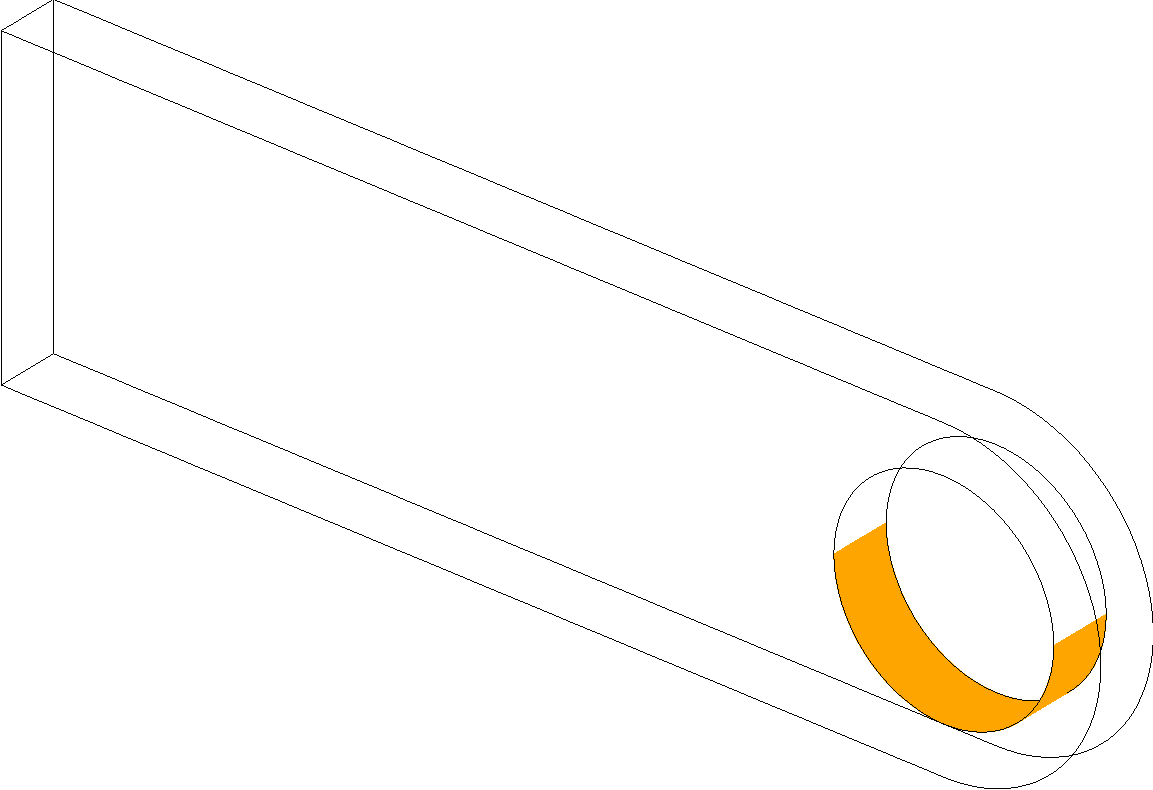
\includegraphics[width=3.5cm]{images/exo/6_cl_force}};
        \begin{scope}[x={(image.south east)},y={(image.north west)}]
          \draw (0.85,0.03) node {\orange{\kw{elmass}}};
        \end{scope}
      \end{tikzpicture}
    \end{textblock*}
    \avous{\fe{Récupérer "la moitié" de \kw{sint} (voir : COOR/POIN/ELEM)}
              {Get the "half part" of \kw{sint} (see: COOR/POIN/ELEM)}}\\
    \avous{\fe{Appliquer une pression (voir : PRES 'MASS')}
              {Apply a pressure (see: PRES 'MASS')}}
    \onslide<6-7>{
      \lstinputlisting[language=gibiane, firstline=100, lastline=104]{dgibi/formation_debutant_3_mecanique.dgibi}}
    \onslide<7>{
      \lstinputlisting[language=gibiane, firstline=105, lastline=105]{dgibi/formation_debutant_3_mecanique.dgibi}
      \lstinputlisting[language=gibiane, firstline=107, lastline=107]{dgibi/formation_debutant_3_mecanique.dgibi}
      \begin{textblock*}{5cm}(7.8cm,-0.5cm)
        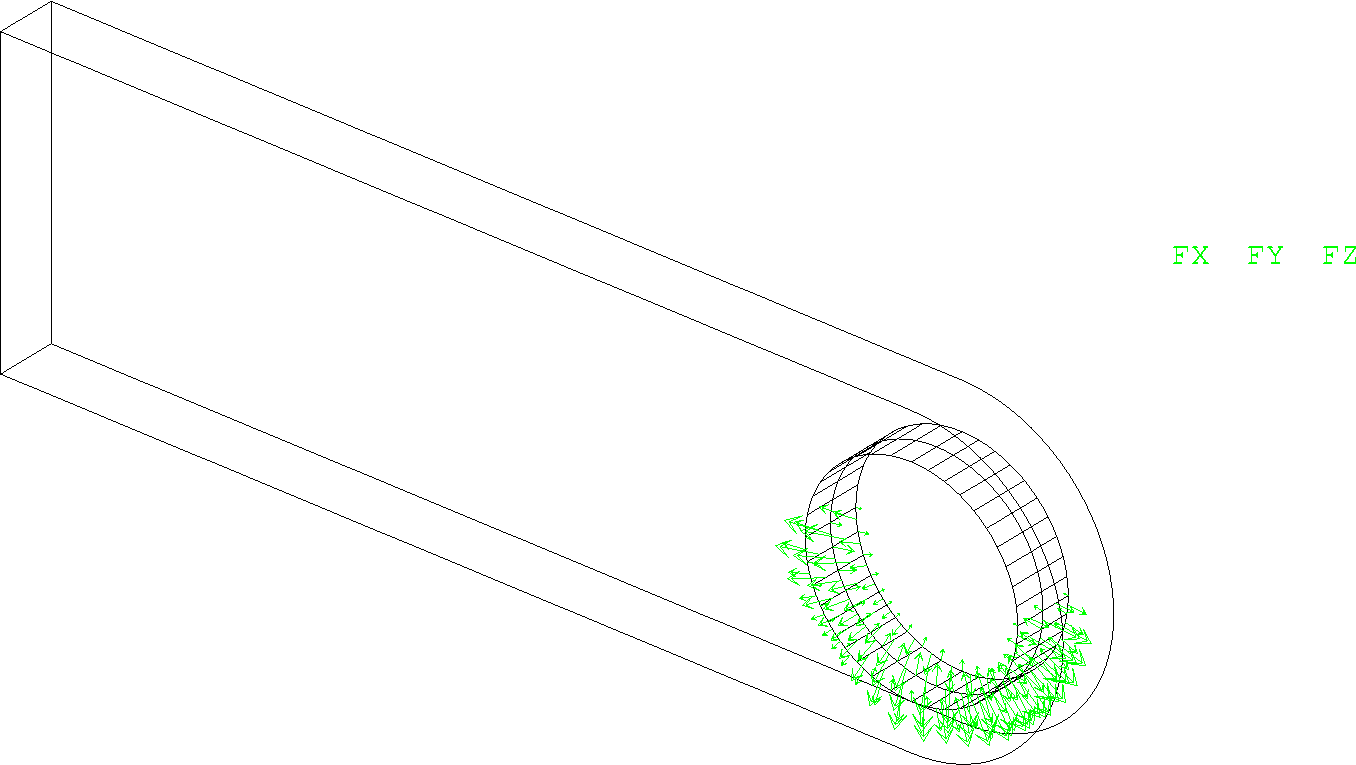
\includegraphics[width=4.5cm]{images/exo/6_forces.2}
      \end{textblock*}}
    \vspace{3cm}
    }
    \only<8-10>{
    \item \fe{3) Avec une \g{\tou{force surfacique}}}{3) With a \g{\tou{surface force}}}\\
    \begin{textblock*}{5cm}(8.7cm,-2.4cm)
      \begin{tikzpicture}
        \scriptsize
        \node[anchor=south west,inner sep=0] (image) at (0,0)
        {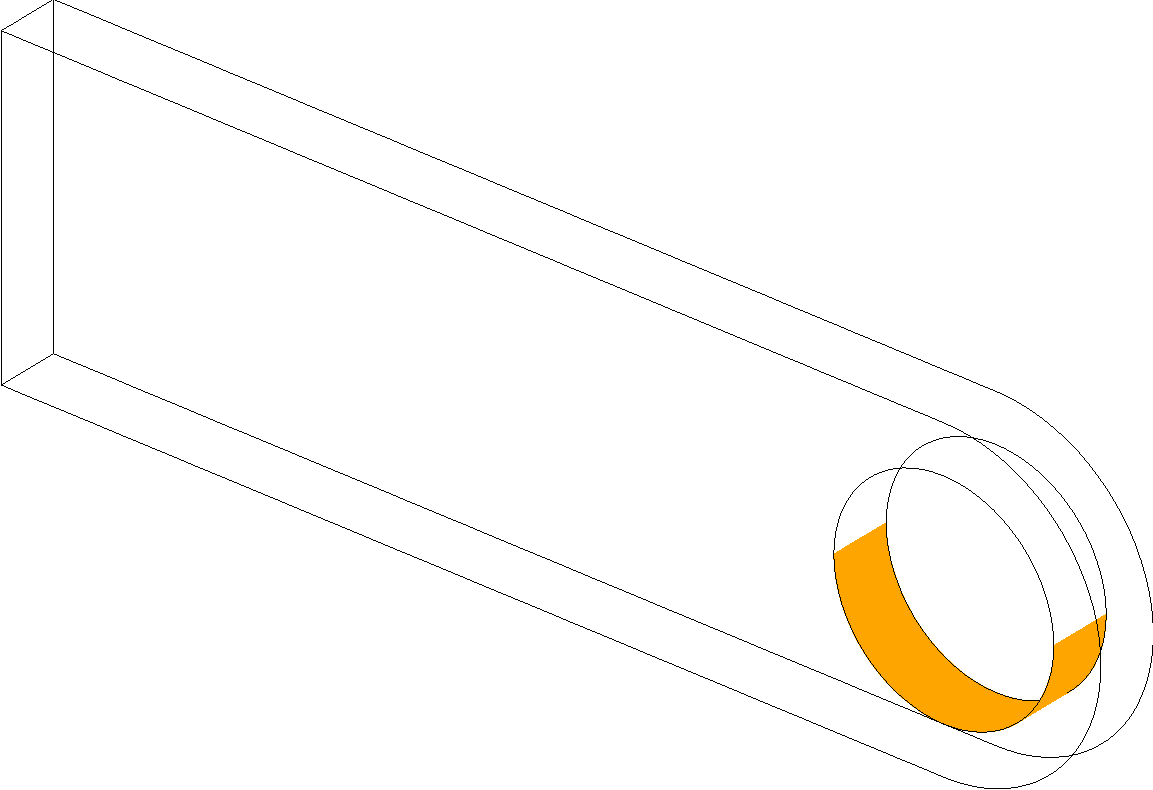
\includegraphics[width=3.5cm]{images/exo/6_cl_force}};
        \begin{scope}[x={(image.south east)},y={(image.north west)}]
          \draw (0.85,0.03) node {\orange{\kw{elmass}}};
        \end{scope}
      \end{tikzpicture}
    \end{textblock*}
    \avous{\fe{Appliquer une force surfacique (voir : FSUR 'MASS')}
              {Apply a surface force (see: FSUR 'MASS')}}
    \onslide<9-10>{
      \lstinputlisting[language=gibiane, firstline=112, lastline=112]{dgibi/formation_debutant_3_mecanique.dgibi}}
    \onslide<10>{
      \lstinputlisting[language=gibiane, firstline=113, lastline=113]{dgibi/formation_debutant_3_mecanique.dgibi}
      \lstinputlisting[language=gibiane, firstline=115, lastline=115]{dgibi/formation_debutant_3_mecanique.dgibi}
      \begin{textblock*}{5cm}(7.8cm,-0.5cm)
        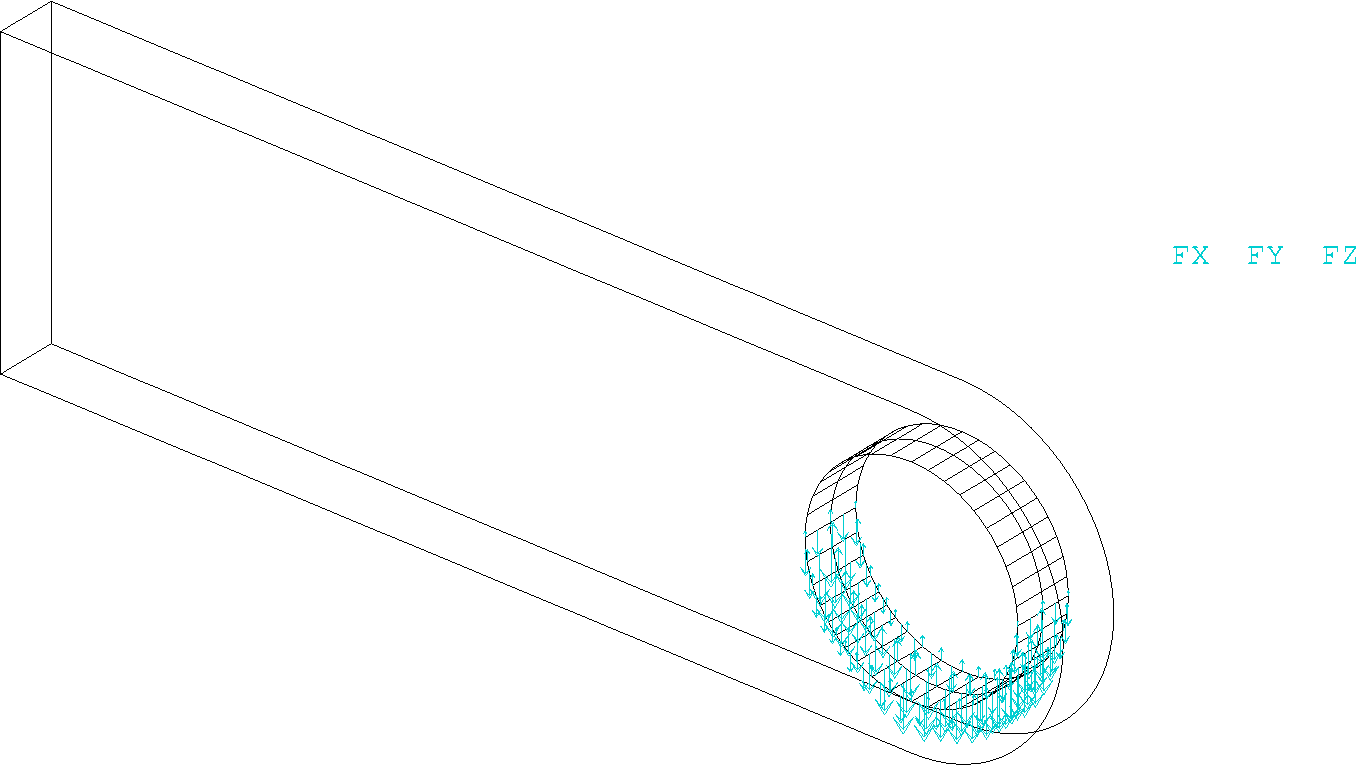
\includegraphics[width=4.5cm]{images/exo/6_forces.3}
      \end{textblock*}}
    \vspace{5cm}
    }
  \end{itemize}
\end{frame}

\begin{frame}{\fe{6 Mécanique linéaire}{6 Linear mechanics}}
             {\fe{Élasticité}{Elasticity}}
  \begin{itemize}
    \item \fe{Résolution des 3 cas de chargement}{Solving 3 load cases}
    \lstinputlisting[basicstyle=\ttfamily\tiny, language=gibiane, firstline=125, lastline=127]{dgibi/formation_debutant_3_mecanique.dgibi}
    \item<2->\fe{Tracé des déformées}{Plotting the deformed shapes}
    \onslide<2->{
      \lstinputlisting[basicstyle=\ttfamily\tiny, language=gibiane, firstline=129, lastline=132]{dgibi/formation_debutant_3_mecanique.dgibi}}
    \onslide<3->{
      \lstinputlisting[basicstyle=\ttfamily\tiny, language=gibiane, firstline=137, lastline=139]{dgibi/formation_debutant_3_mecanique.dgibi}}
    \onslide<3>{
      \begin{textblock*}{5cm}(8.7cm,-6.2cm)
        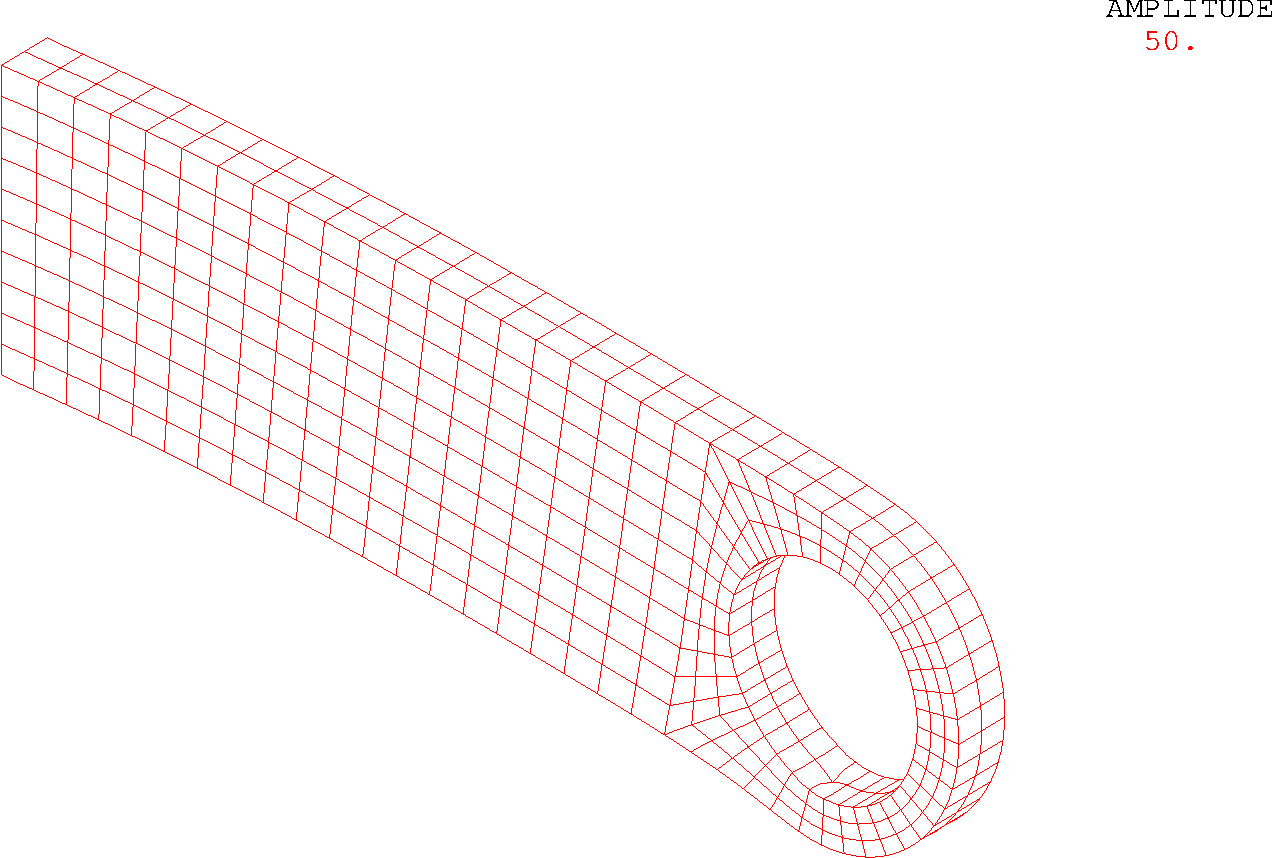
\includegraphics[width=3.6cm]{images/exo/6_deformees.1}
      \end{textblock*}
      \begin{textblock*}{5cm}(8.7cm,-3.4cm)
        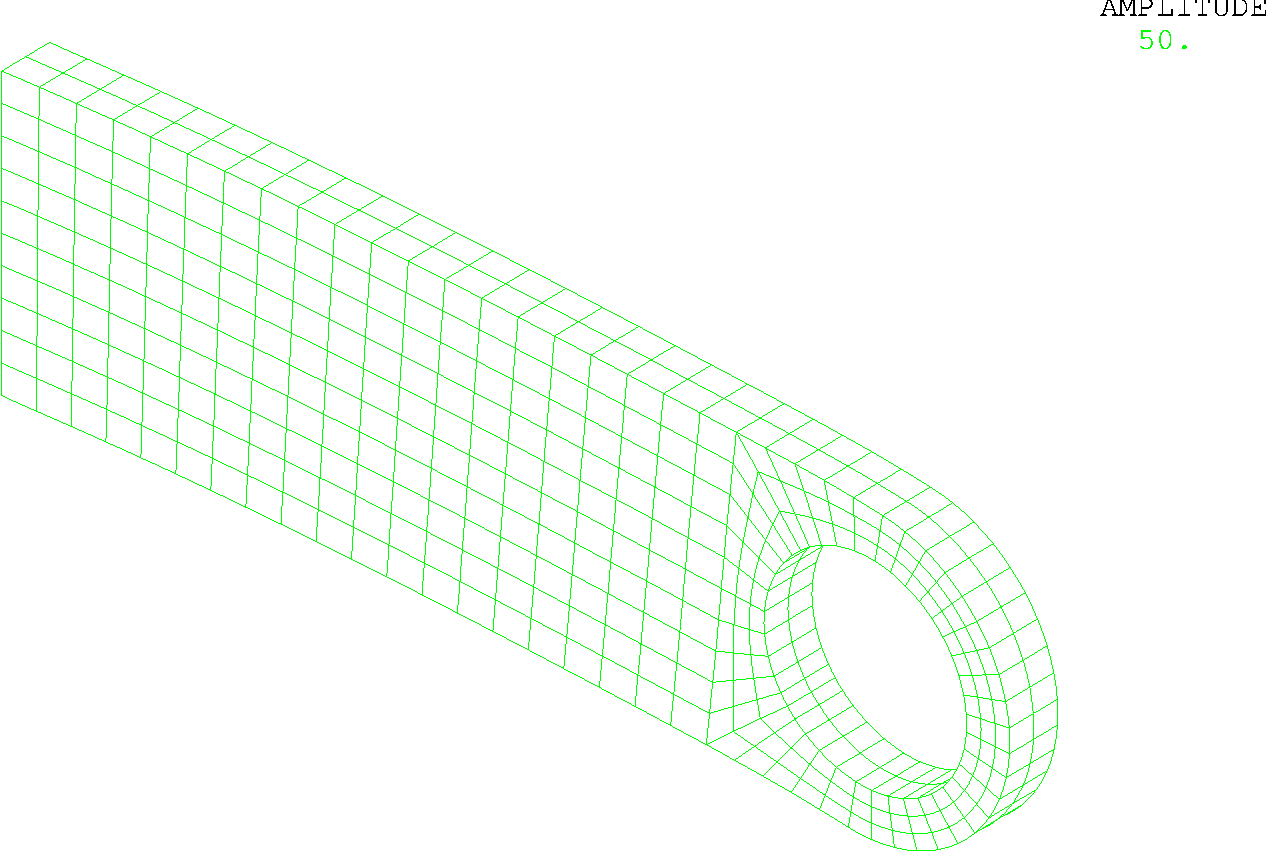
\includegraphics[width=3.6cm]{images/exo/6_deformees.2}
      \end{textblock*}
      \begin{textblock*}{5cm}(8.7cm,-0.6cm)
        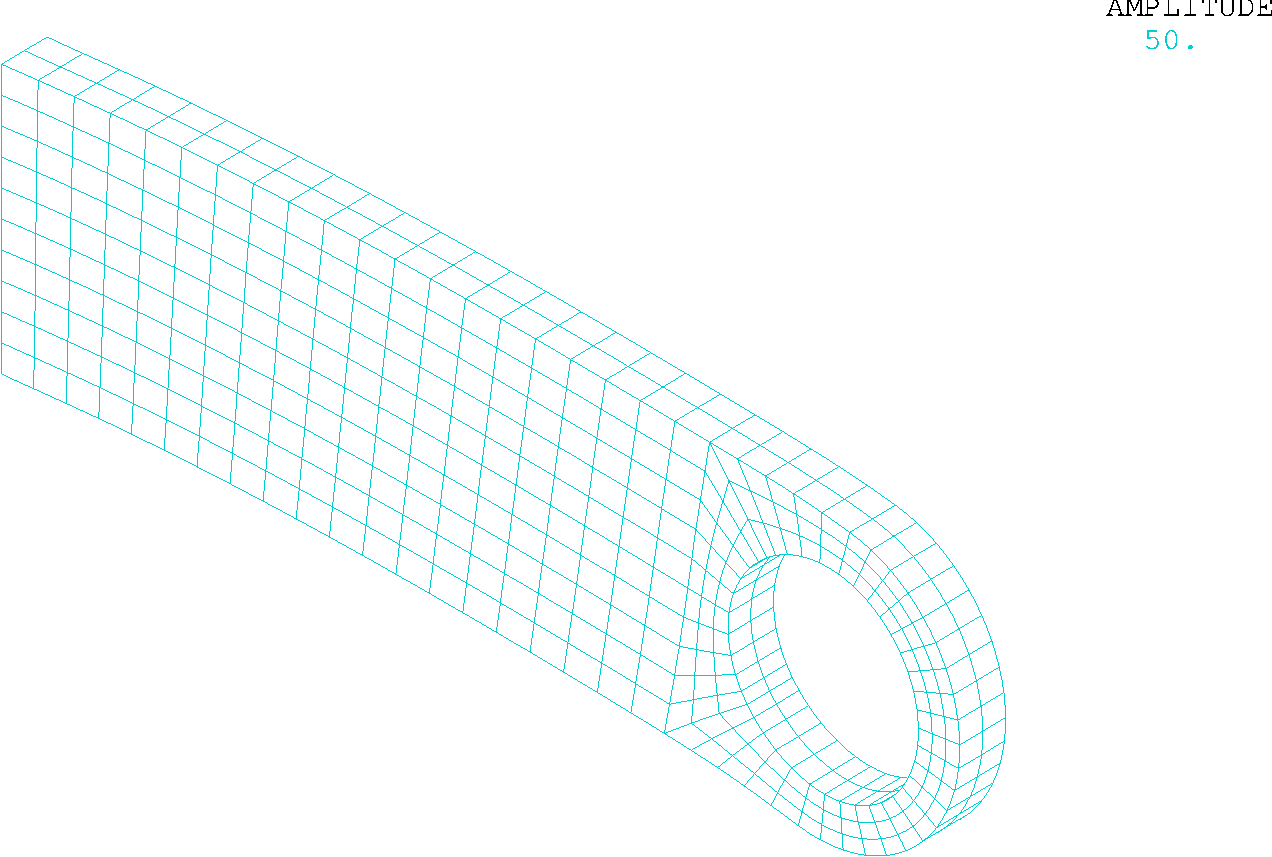
\includegraphics[width=3.6cm]{images/exo/6_deformees.3}
      \end{textblock*}}
    \onslide<4->{
      \lstinputlisting[basicstyle=\ttfamily\tiny, language=gibiane, firstline=141, lastline=143]{dgibi/formation_debutant_3_mecanique.dgibi}
      \lstinputlisting[basicstyle=\ttfamily\tiny, language=gibiane, firstline=145, lastline=145]{dgibi/formation_debutant_3_mecanique.dgibi}
      \begin{textblock*}{5.5cm}(6.5cm,-3cm)
        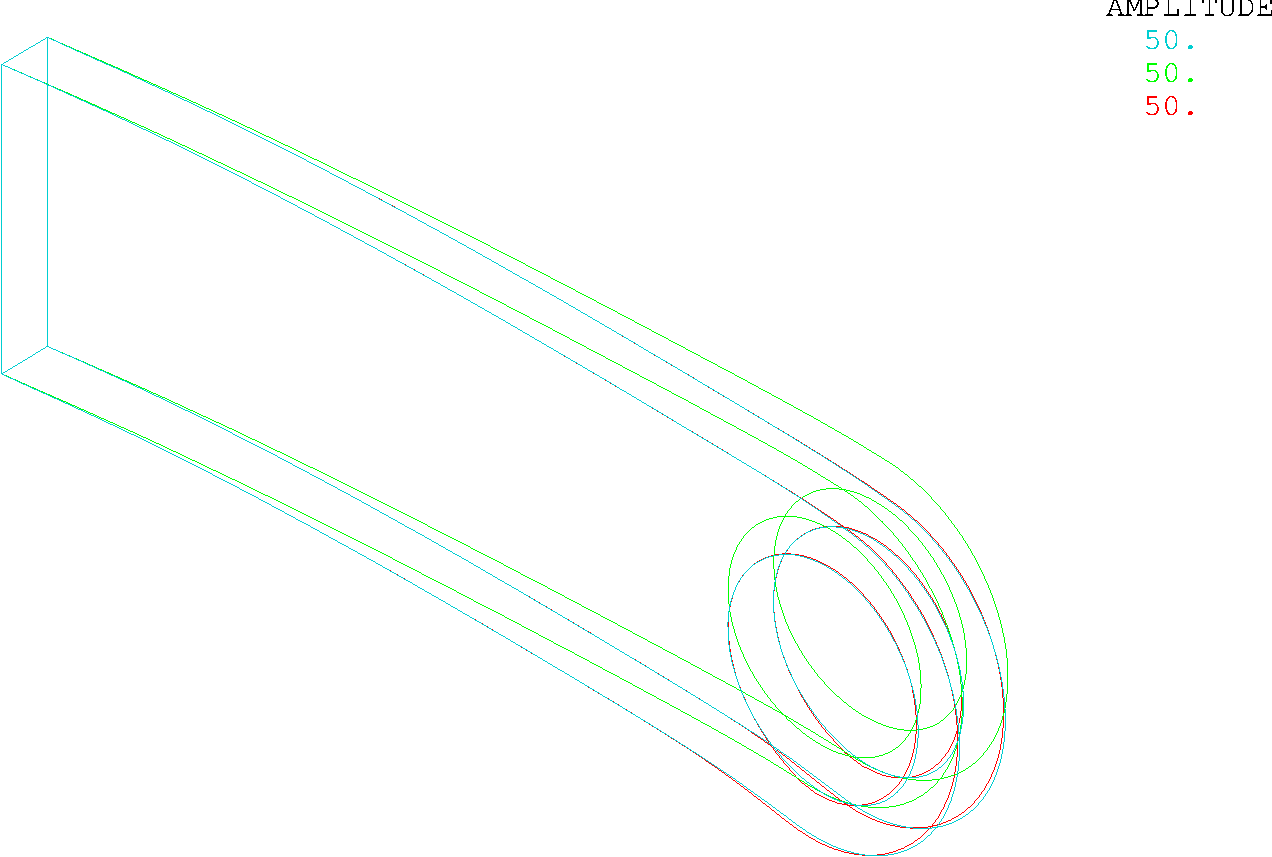
\includegraphics[width=5.5cm]{images/exo/6_deformees.4}
      \end{textblock*}}
  \end{itemize}
\end{frame}

\begin{frame}{\fe{6 Mécanique linéaire}{6 Linear mechanics}}
             {\fe{Élasticité}{Elasticity}}
  \begin{itemize}
    \item \fe{Forces de réaction}{Reaction forces}
    \lstinputlisting[basicstyle=\ttfamily\tiny, language=gibiane, firstline=148, lastline=150]{dgibi/formation_debutant_3_mecanique.dgibi}
    \lstinputlisting[basicstyle=\ttfamily\tiny, language=gibiane, firstline=155, lastline=155]{dgibi/formation_debutant_3_mecanique.dgibi}
    \begin{textblock*}{5cm}(7.4cm,-2.5cm)
      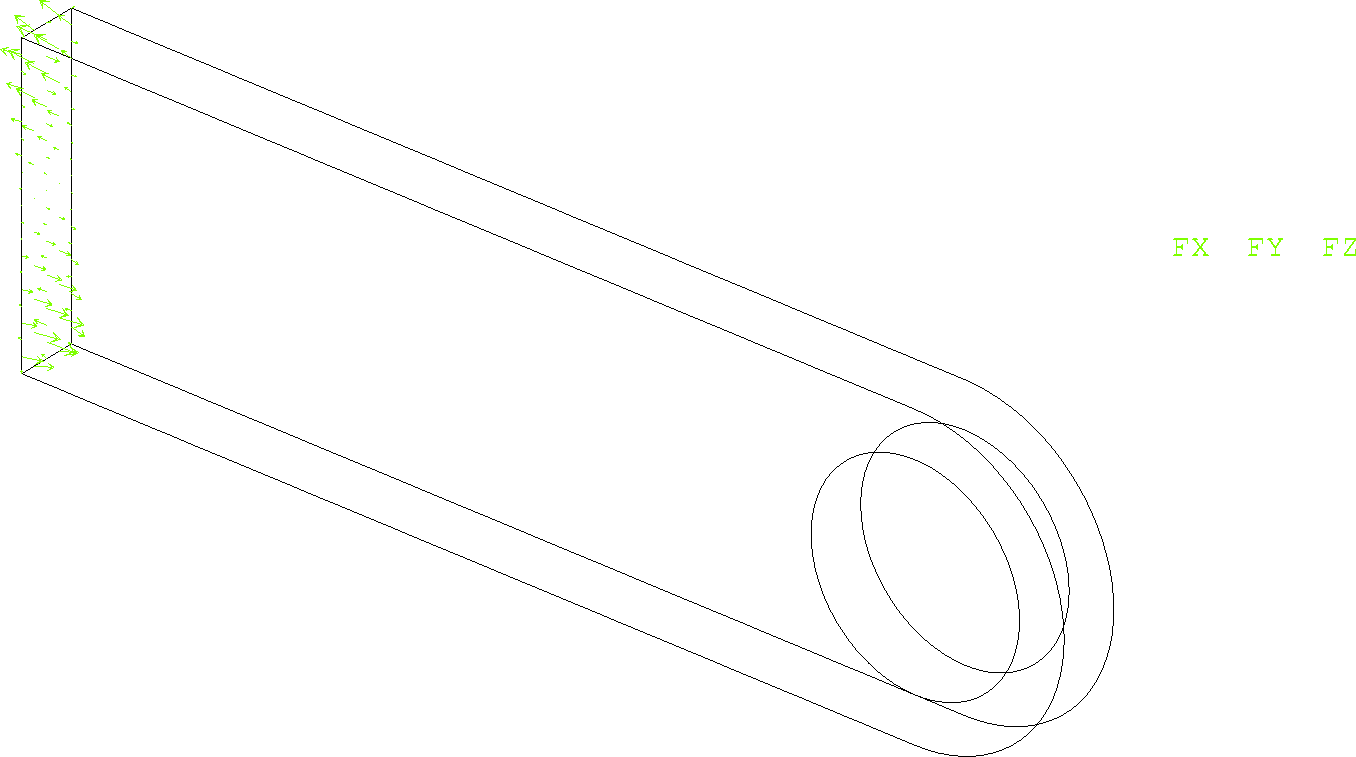
\includegraphics[width=5cm]{images/exo/6_reactions}
    \end{textblock*}
    \item<2->\fe{Déformations et contraintes}{Strains and stresses}
    \onslide<2->{
      \lstinputlisting[basicstyle=\ttfamily\tiny, language=gibiane, firstline=158, lastline=162]{dgibi/formation_debutant_3_mecanique.dgibi}
      \lstinputlisting[basicstyle=\ttfamily\tiny, language=gibiane, firstline=167, lastline=167]{dgibi/formation_debutant_3_mecanique.dgibi}}
    \onslide<2>{
      \begin{textblock*}{5cm}(7.4cm,-2cm)
        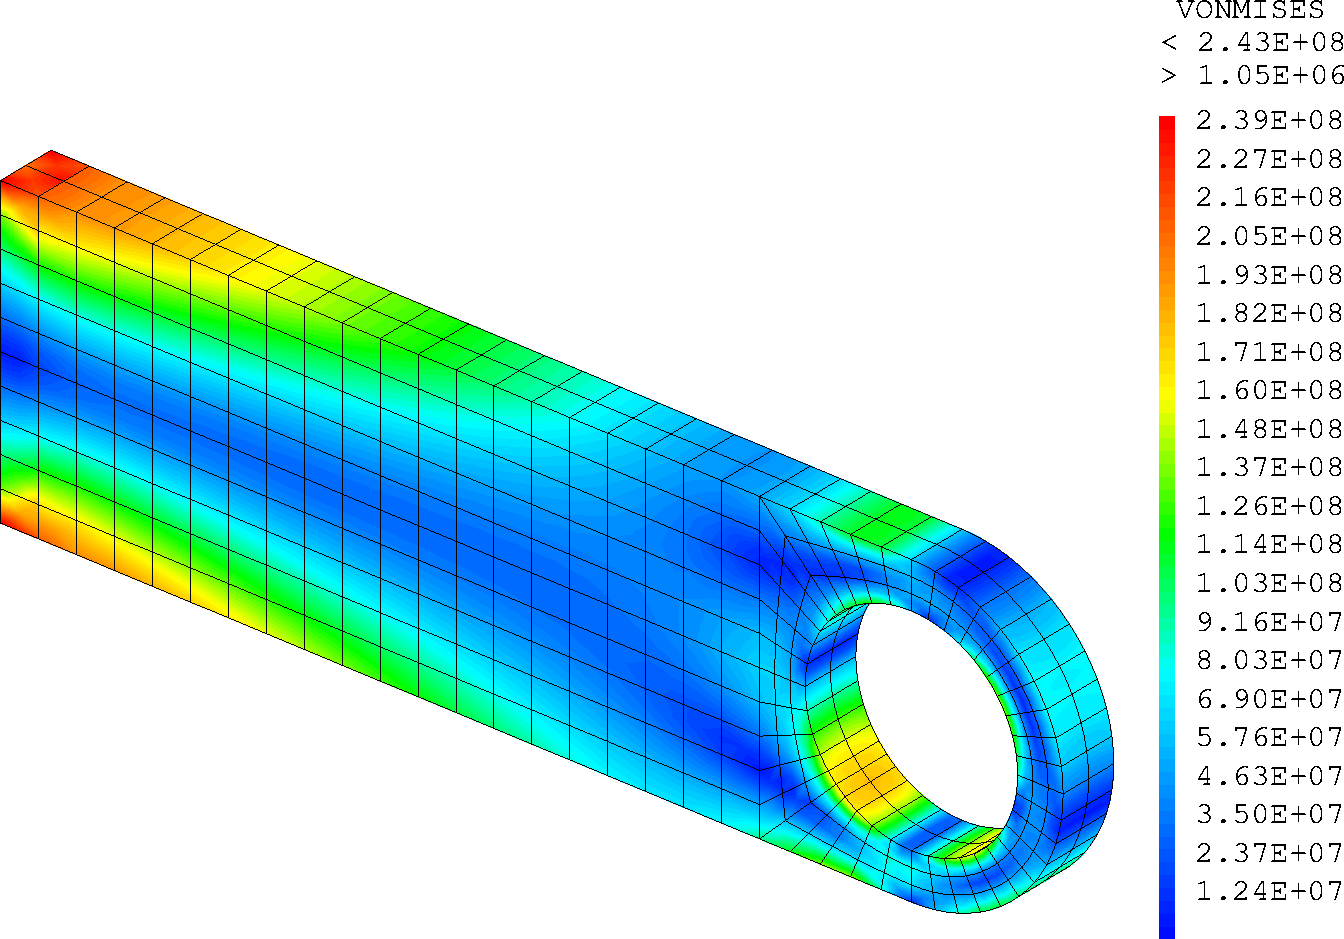
\includegraphics[width=5cm]{images/exo/6_contraintes.1.pdf}
      \end{textblock*}}
    \onslide<3>{
      \begin{textblock*}{5cm}(7.4cm,-2cm)
        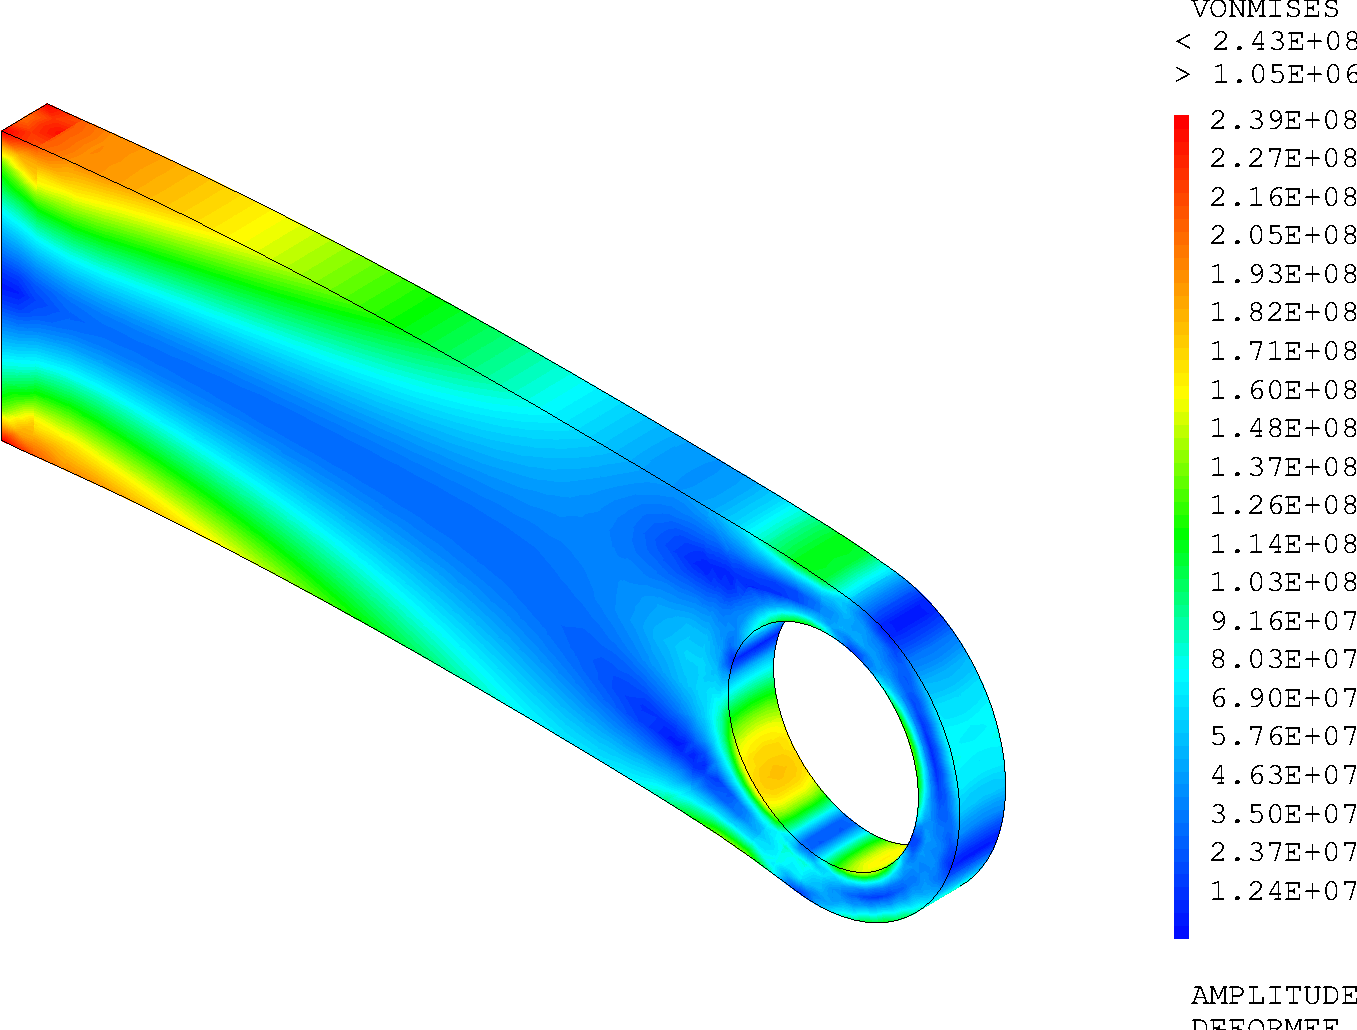
\includegraphics[width=5cm]{images/exo/6_contraintes.2.pdf}
      \end{textblock*}}
    \onslide<3->{
      \lstinputlisting[basicstyle=\ttfamily\tiny, language=gibiane, firstline=169, lastline=169]{dgibi/formation_debutant_3_mecanique.dgibi}
      \lstinputlisting[basicstyle=\ttfamily\tiny, language=gibiane, firstline=171, lastline=171]{dgibi/formation_debutant_3_mecanique.dgibi}
      \vspace{0.5cm}
      \item[]<3-> \violet{\emph{\fe{Nouvel objet : DEFORMEE}{New object: DEFORMEE}}}}
  \end{itemize}
\end{frame}

\begin{frame}{\fe{6 Mécanique linéaire}{6 Linear mechanics}}
             {\fe{Élasticité}{Elasticity}}
  \begin{itemize}
    \item \fe{Contrainte de von Mises}{von Mises stress}
    \lstinputlisting[basicstyle=\ttfamily\tiny, language=gibiane, firstline=174, lastline=176]{dgibi/formation_debutant_3_mecanique.dgibi}
    \lstinputlisting[basicstyle=\ttfamily\tiny, language=gibiane, firstline=178, lastline=178]{dgibi/formation_debutant_3_mecanique.dgibi}
    \begin{textblock*}{5cm}(7.4cm,-4cm)
      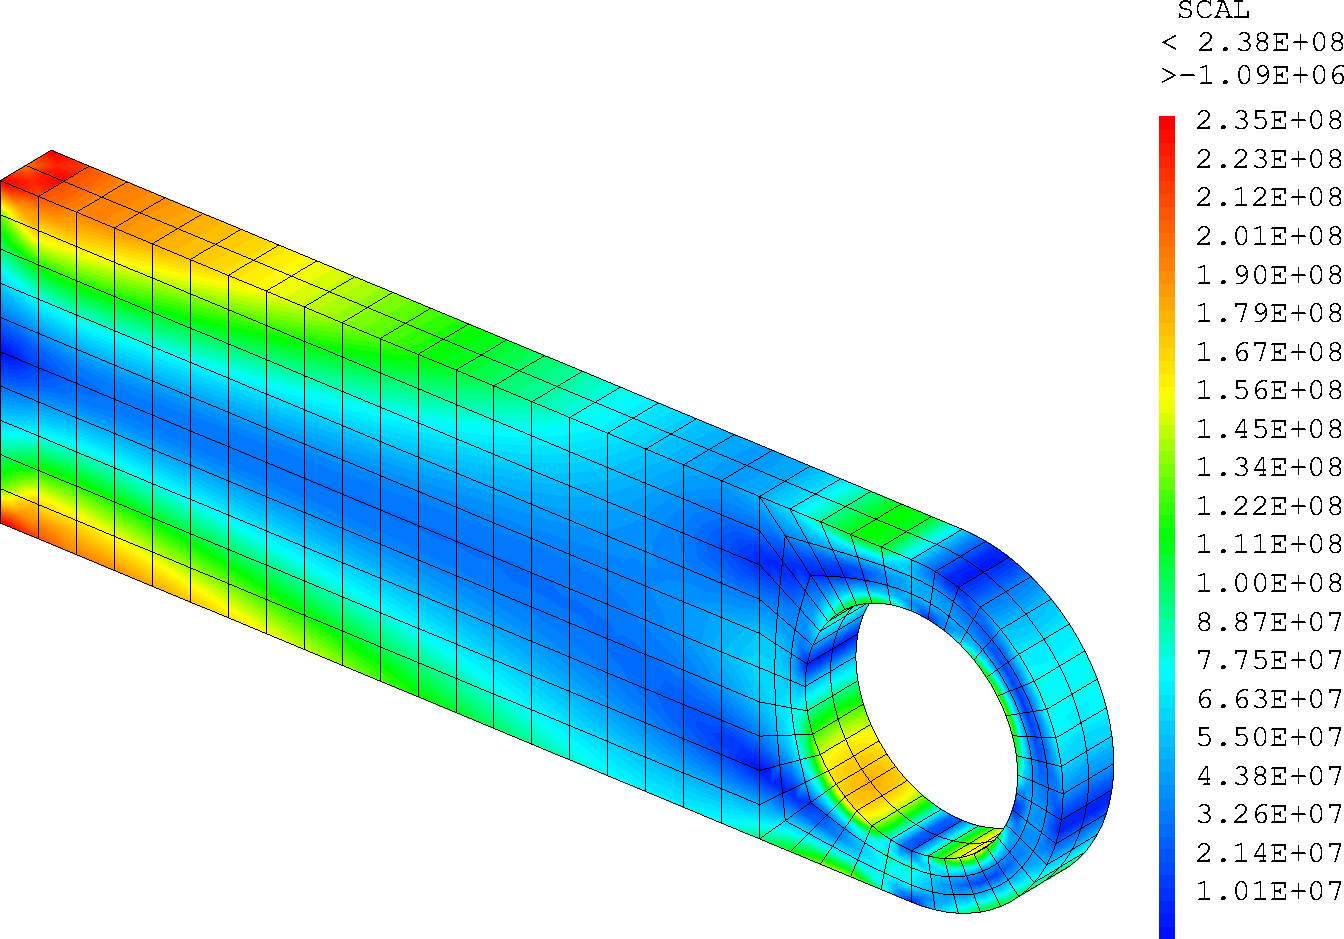
\includegraphics[width=5cm]{images/exo/6_contraintes.3.pdf}
    \end{textblock*}
    \onslide<2->{
      \lstinputlisting[basicstyle=\ttfamily\tiny, language=gibiane, firstline=180, lastline=180]{dgibi/formation_debutant_3_mecanique.dgibi}
      \lstinputlisting[basicstyle=\ttfamily\tiny, language=gibiane, firstline=182, lastline=182]{dgibi/formation_debutant_3_mecanique.dgibi}
      \begin{textblock*}{5cm}(7.4cm,-1.1cm)
        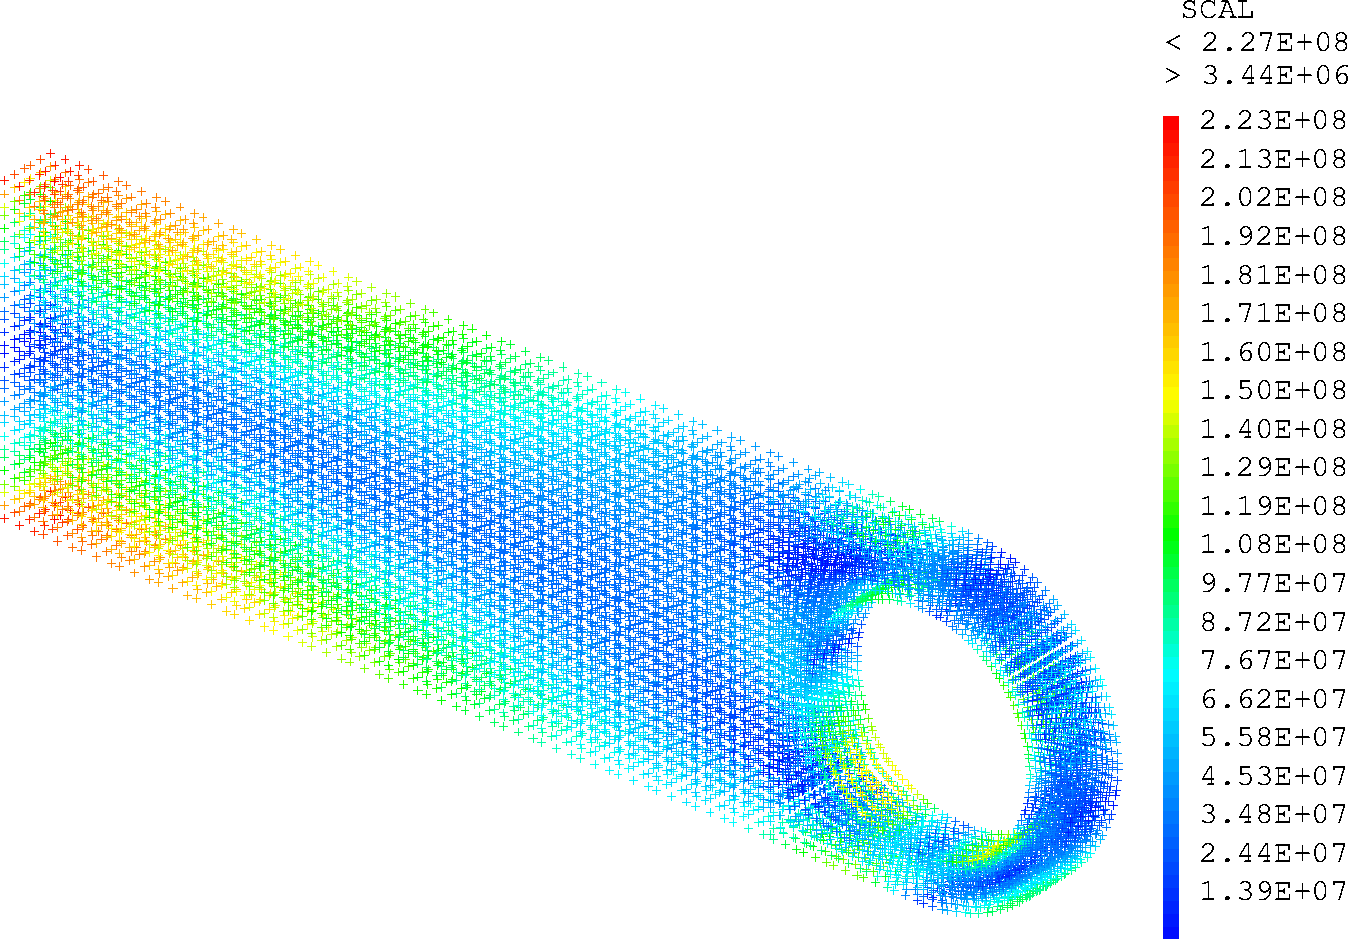
\includegraphics[width=5cm]{images/exo/6_contraintes.4.pdf}
      \end{textblock*}}
  \end{itemize}
\end{frame}

\begin{frame}{\fe{6 Mécanique linéaire}{6 Linear mechanics}}
             {\fe{Élasticité}{Elasticity}}
  \begin{itemize}
    \item \fe{Évolution d'un champ le long d'une ligne\\
              du maillage}
             {Field evolution along a line of the mesh\\~}
    \lstinputlisting[basicstyle=\ttfamily\tiny, language=gibiane, firstline=185, lastline=188]{dgibi/formation_debutant_3_mecanique.dgibi}
    \lstinputlisting[basicstyle=\ttfamily\tiny, language=gibiane, firstline=193, lastline=193]{dgibi/formation_debutant_3_mecanique.dgibi}
    \begin{textblock*}{5cm}(8.1cm,-2.7cm)
      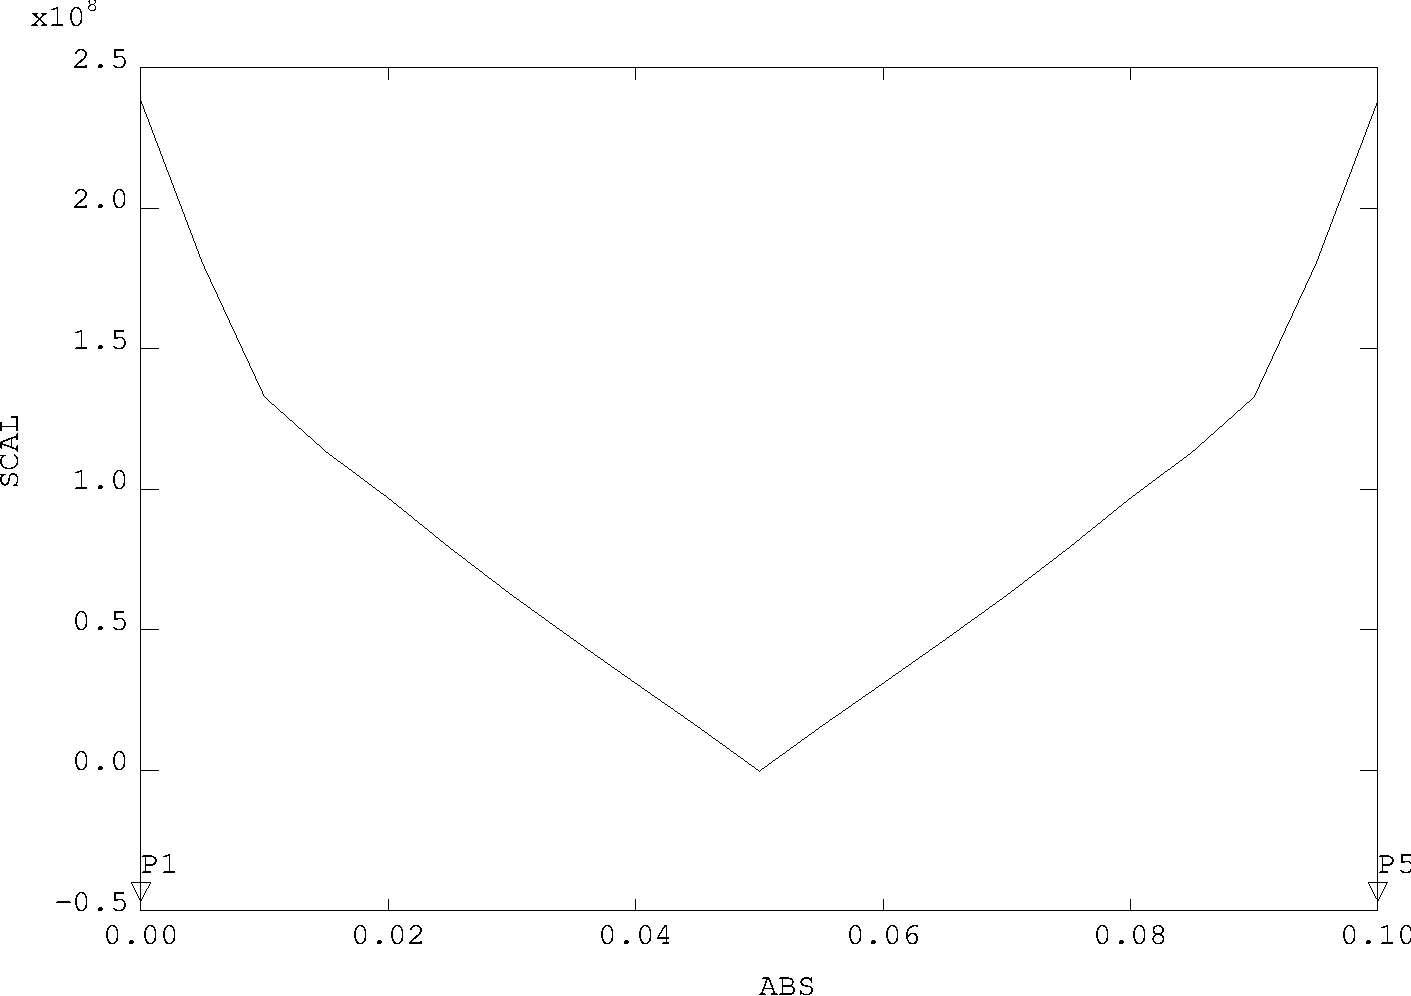
\includegraphics[width=4cm]{images/exo/6_evol_contraintes.1}
    \end{textblock*}
    \item<2->\fe{Évolution d'un champ le long d'une ligne\\
                 quelconque}
                {Field evolution along any line\\~}
    \onslide<2->{
      \lstinputlisting[basicstyle=\ttfamily\tiny, language=gibiane, firstline=196, lastline=202]{dgibi/formation_debutant_3_mecanique.dgibi}
      \lstinputlisting[basicstyle=\ttfamily\tiny, language=gibiane, firstline=204, lastline=204]{dgibi/formation_debutant_3_mecanique.dgibi}
      \begin{textblock*}{5cm}(8.6cm,-3.3cm)
        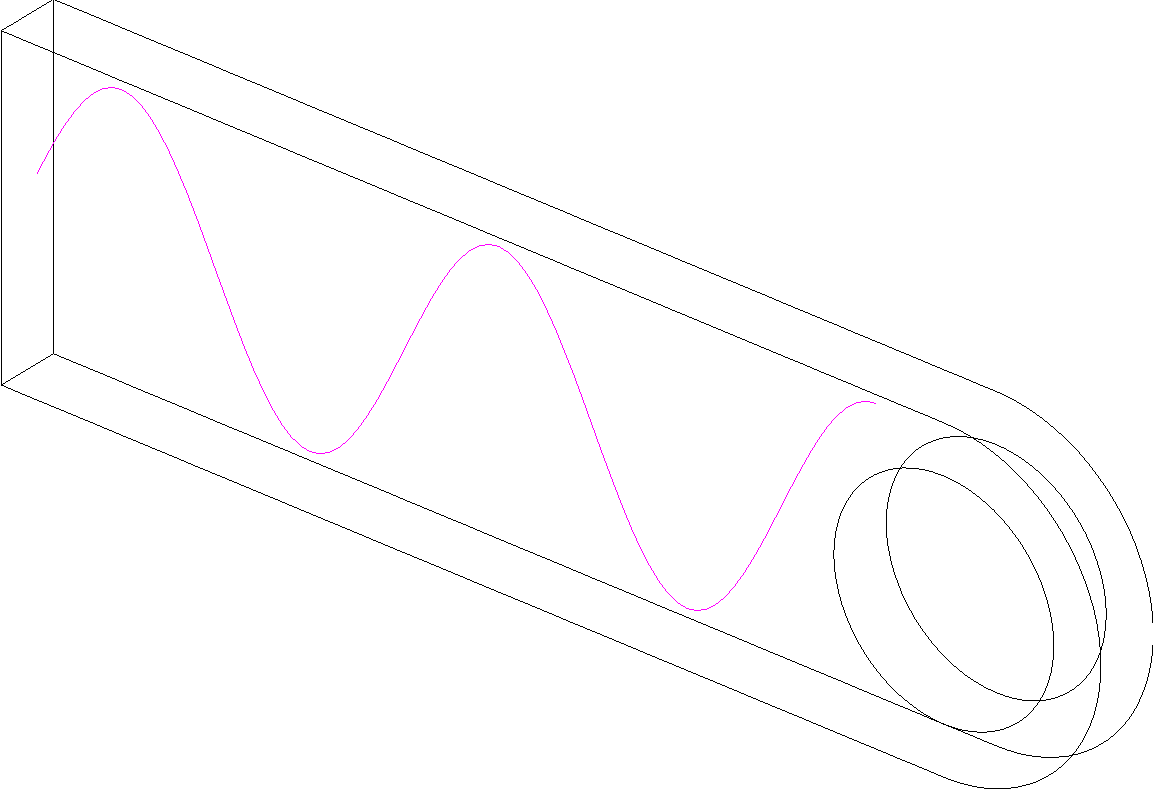
\includegraphics[width=3cm]{images/exo/6_evol_contraintes.2}
      \end{textblock*}}
    \onslide<3->{
      \lstinputlisting[basicstyle=\ttfamily\tiny, language=gibiane, firstline=206, lastline=208]{dgibi/formation_debutant_3_mecanique.dgibi}
      \lstinputlisting[basicstyle=\ttfamily\tiny, language=gibiane, firstline=210, lastline=210]{dgibi/formation_debutant_3_mecanique.dgibi}
      \begin{textblock*}{5cm}(8.1cm,-2.7cm)
        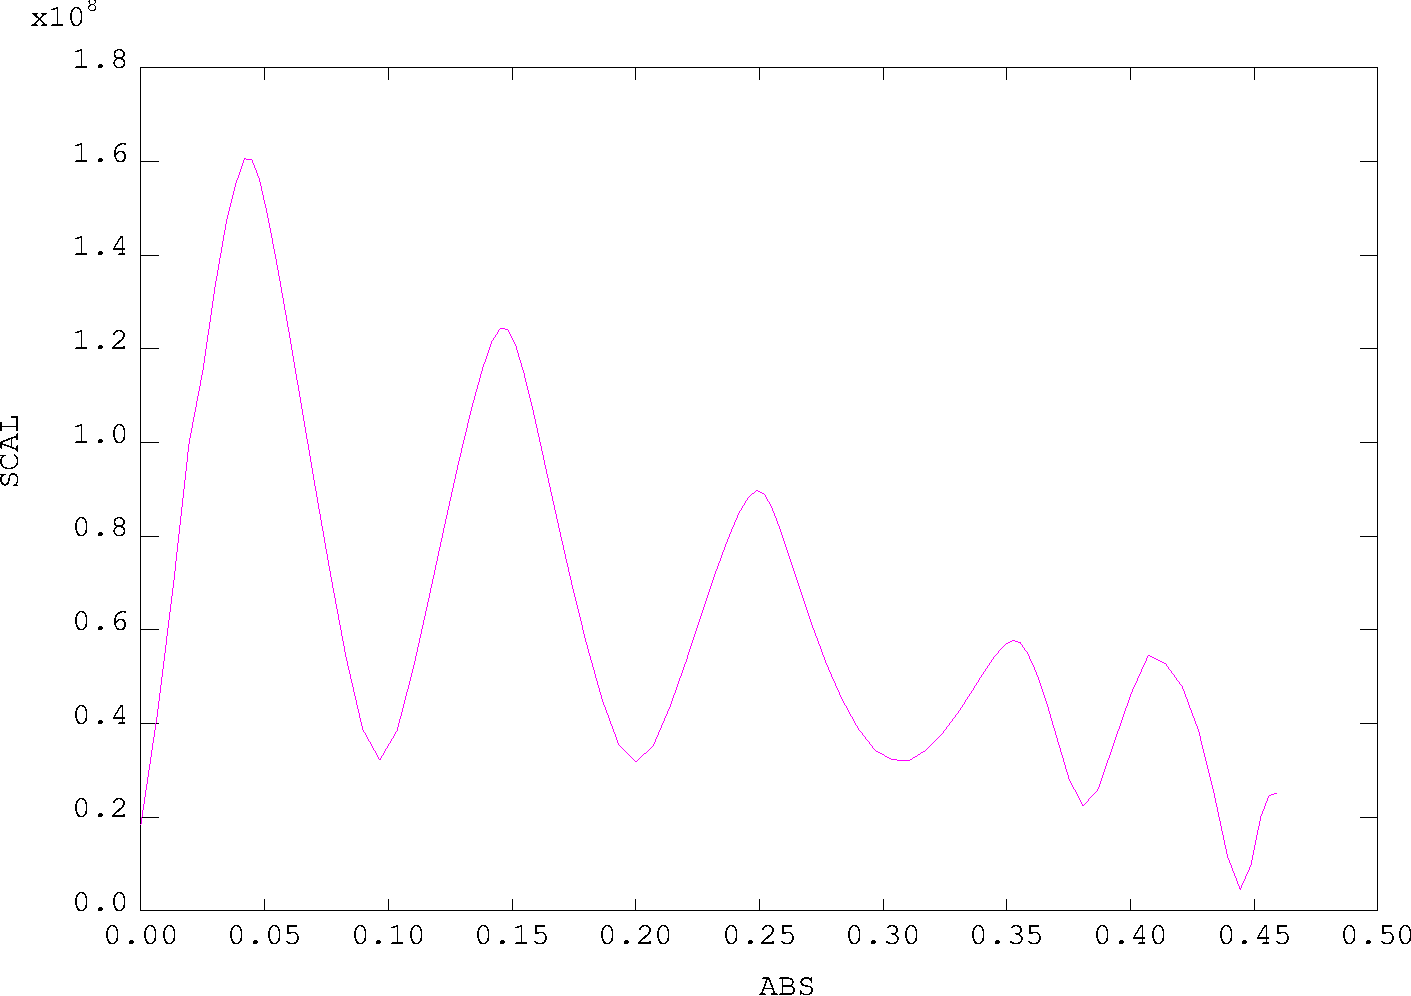
\includegraphics[width=4cm]{images/exo/6_evol_contraintes.3}
      \end{textblock*}}
  \end{itemize}
\end{frame}





\fe{\subsection{Thermo Mécanique linéaire}}{\subsection{Linear Thermo Mechanics}}
\begin{frame}{\fe{7 Problème étudié}{7 Problem description}}
  \begin{itemize}
    \item \gray{\fe{Élasticité linéaire}{Linear elasticity}}
    \begin{columns}
      \begin{column}{.4\textwidth}
        \item \gray{\fe{Déplacements imposés}{Imposed displacements}}
        \footnotesize
        \begin{tikzpicture}
          \node[anchor=south west,inner sep=0,opacity=0.3] (image) at (0,0)
          {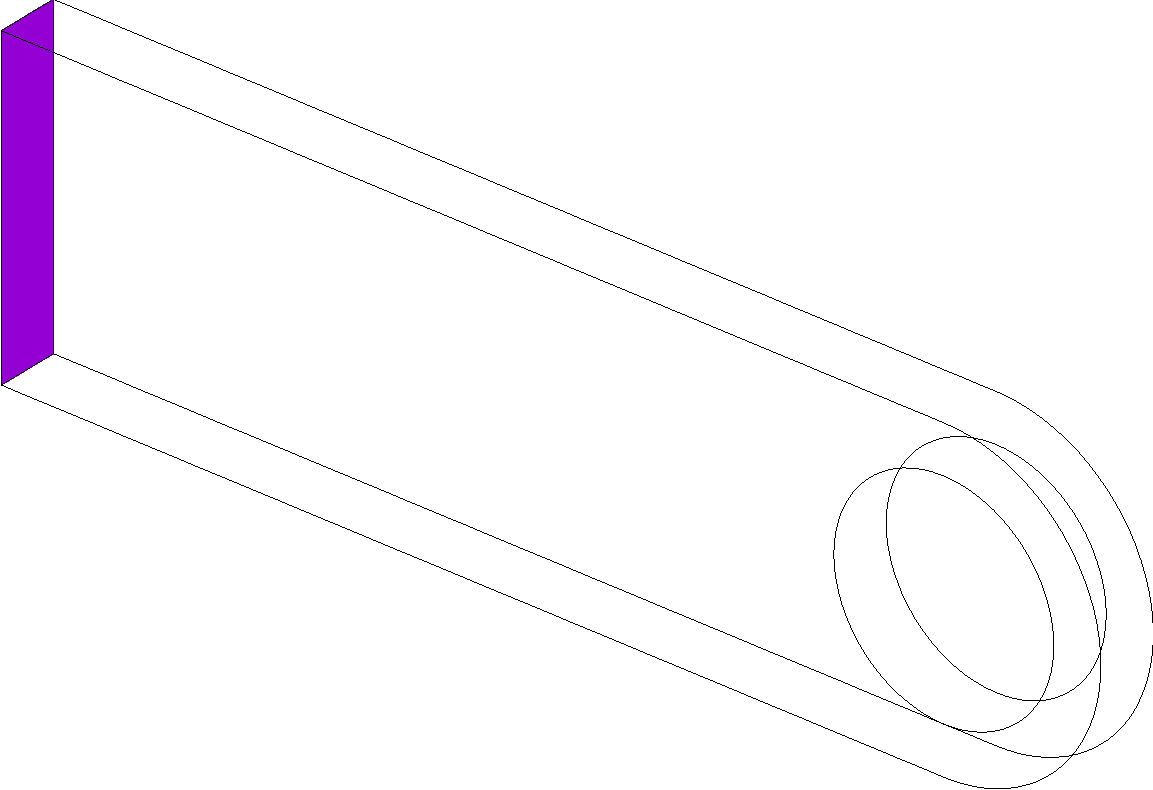
\includegraphics[width=3.5cm]{images/exo/6_cl_deplacement}};
          \begin{scope}[x={(image.south east)},y={(image.north west)},color=violet,opacity=0.3]
            \draw (0.06,0.7) node[anchor=north west] {$u_x=u_y=u_z$~=~0~m};
          \end{scope}
        \end{tikzpicture}
        \normalsize
      \end{column}
      \begin{column}{.4\textwidth}
        \item \gray{\fe{Forces imposées}{Imposed forces}}
        \footnotesize
        \begin{tikzpicture}
          \node[anchor=south west,inner sep=0,opacity=0.3] (image) at (0,0)
          {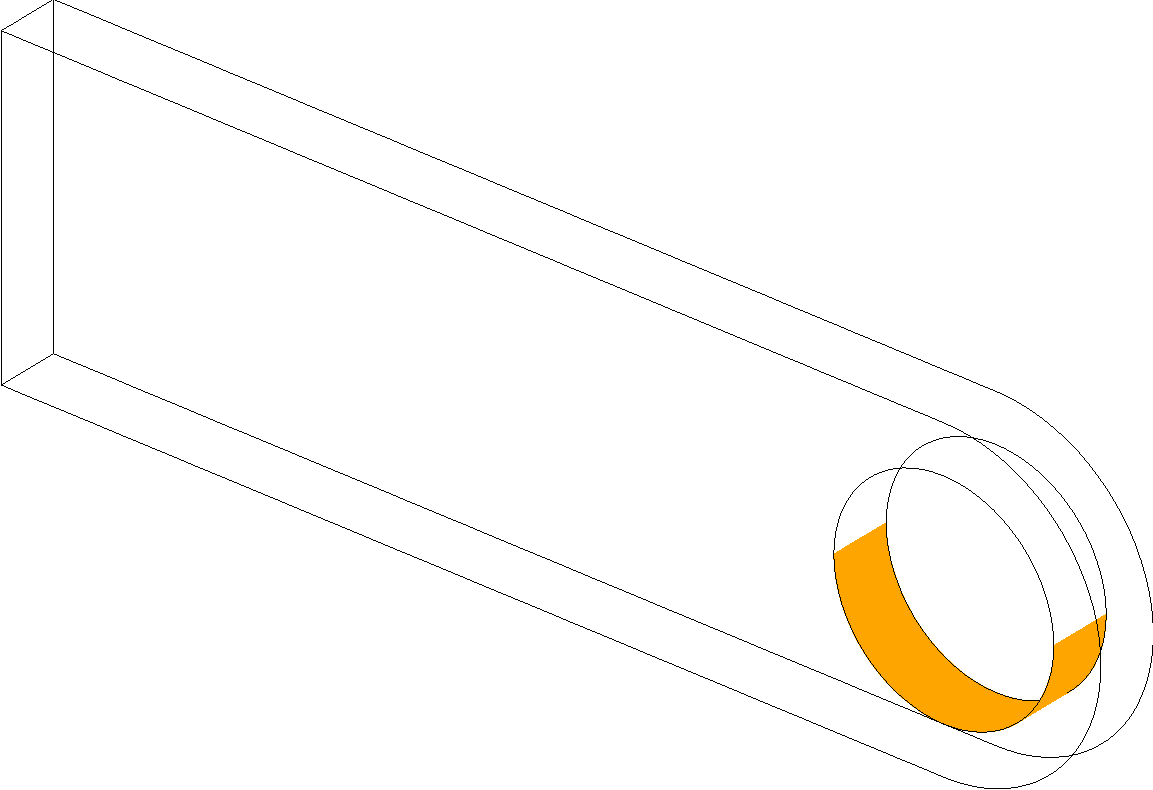
\includegraphics[width=3.5cm]{images/exo/6_cl_force}};
          \begin{scope}[x={(image.south east)},y={(image.north west)},color=orange,opacity=0.3]
            \draw (0.8,0.75) node[anchor=north west] {\fe{masse suspendue}{hanging mass}};
            \draw (0.9,0.6) node[anchor=north west] {$m$~=~2500~kg};
          \end{scope}
        \end{tikzpicture}
        \normalsize
      \end{column}
    \end{columns}
    \begin{columns}
      \begin{column}{.4\textwidth}
        \item \fe{\tou{Chargement thermique}}{\tou{Thermal load}}
        \footnotesize
        \begin{tikzpicture}
          \node[anchor=south west,inner sep=0] (image) at (0,0)
          {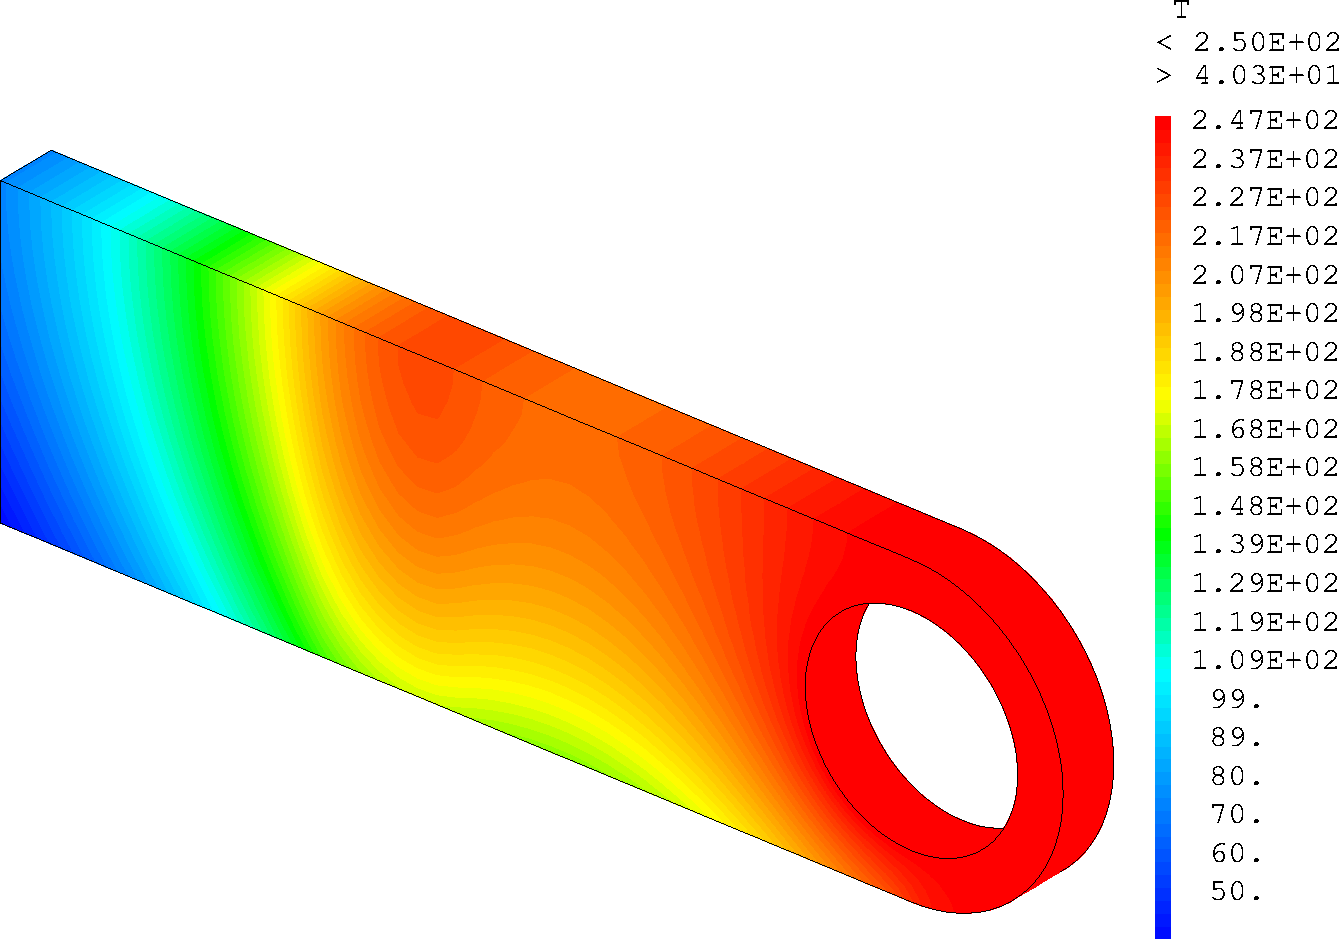
\includegraphics[width=4cm]{images/exo/2.2_temperatures}};
          \begin{scope}[x={(image.south east)},y={(image.north west)},color=blue]
            \draw (0.1,0.2) node {dilatation};
            \draw (0.1,0.05) node {$\alpha$~=~10$^{-5}$~K$^{-1}$};
          \end{scope}
        \end{tikzpicture}
        \normalsize
      \end{column}
      \begin{column}{.4\textwidth}
      \end{column}
    \end{columns}
  \end{itemize}
\end{frame}

\begin{frame}{\fe{7 Mécanique linéaire}{7 Linear mechanics}}
             {\fe{Élasticité, chargement thermique}{Elasticity, thermal load}}
  \begin{itemize}
    \item \fe{Prise en compte de la dilatation thermique}
             {Taking thermal expansion into account}
    \begin{equation*}
      \int_{V}[B]^T\{\sigma\}dV=\{F\}
    \end{equation*}
    \begin{equation*}
      \int_{V}[B]^T[C]\{\varepsilon-\green{\varepsilon_{\tx{th}}}\}dV=\{F\}
    \end{equation*}
    \begin{equation*}
      \int_{V}[B]^T[C]\{\varepsilon\}dV=\{F\}+\green{\int_{V}[B]^T[C]\{\varepsilon\}_{\tx{th}}dV}
    \end{equation*}
    \begin{equation*}
      [K]\{U\}=\{F\}+\green{\underbrace{\int_{V}[B]^T[C]\{\varepsilon\}_{\tx{th}}dV}_{\{F\}_{\tx{th}}}}
    \end{equation*}
  \end{itemize}
\end{frame}

\begin{frame}{\fe{7 Mécanique linéaire}{7 Linear mechanics}}
             {\fe{Élasticité, chargement thermique}{Elasticity, thermal load}}
  \begin{itemize}
    \item \fe{Objectif : calcul mécanique linéaire précédent\\
              \tou{avec un chargement thermique supplémentaire}}
            {Objective: previous linear mechanical calculation\\
             \tou{with an additional thermal load}}
    \begin{equation*}
      [K]\{U\}=\{F\}+\green{\underbrace{\int_{V}[B]^T[C]\{\varepsilon\}_{\tx{th}}dV}_{\{F\}_{\tx{th}}}}
    \end{equation*}
    \item \fe{Méthode :}{Method:}\\
    \begin{tabular}{ll}
      \fe{déformations thermiques}{thermal strains} & $\green{\{\varepsilon\}_{\tx{th}}}$\\
      \fe{contraintes thermiques}{thermal stresses} & $\green{\{\sigma\}_{\tx{th}}=[C]\{\varepsilon\}_{\tx{th}}}$\\
      \fe{forces nodales éq.}{nodal eq. forces} & $\green{\{F\}_{\tx{th}}=\int_{V}[B]^T\{\sigma\}_{\tx{th}}dV}$\\
      \fe{résolution avec \kwr{RESO}}{sovling with \kwr{RESO}} & $\{U\}=[K]^{-1}(\{F\}+\green{\{F\}_{\tx{th}}})$
    \end{tabular}
  \end{itemize}
\end{frame}

\begin{frame}{\fe{7 Mécanique linéaire}{7 Linear mechanics}}
             {\fe{Élasticité, chargement thermique}{Elasticity, thermal load}}
  \begin{itemize}
    \item \fe{Déformation thermique}{Thermal strain}
    \lstinputlisting[language=gibiane, firstline=229, lastline=232]{dgibi/formation_debutant_3_mecanique.dgibi}
    \begin{flushright}
      \footnotesize
      $\{\varepsilon\}_{\tx{th}}=\alpha\{\Delta T\}$
      \normalsize
    \end{flushright}
    \item \fe{Pseudo contraintes thermique}{Pseudo thermal stresses}
    \lstinputlisting[language=gibiane, firstline=234, lastline=235]{dgibi/formation_debutant_3_mecanique.dgibi}
    \begin{flushright}
      \footnotesize
      $\{\sigma\}_{\tx{th}}=[C]\{\varepsilon\}_{\tx{th}}$
      \normalsize
    \end{flushright}
    \item \fe{Forces nodale équivalentes}{Nodal equivalent forces}
    \lstinputlisting[language=gibiane, firstline=237, lastline=239]{dgibi/formation_debutant_3_mecanique.dgibi}
    \begin{flushright}
      \footnotesize
      $\{F\}_{\tx{th}}=\int_{V}[B]^T\{\sigma\}_{\tx{th}}dV$
      \normalsize
    \end{flushright}
  \end{itemize}
\end{frame}

\begin{frame}{\fe{7 Mécanique linéaire}{7 Linear mechanics}}
             {\fe{Élasticité, chargement thermique}{Elasticity, thermal load}}
  \begin{itemize}
    \item \fe{Résolution et affichage des résultats}{Solving and plotting results}
    \lstinputlisting[language=gibiane, firstline=241, lastline=246]{dgibi/formation_debutant_3_mecanique.dgibi}
    \lstinputlisting[language=gibiane, firstline=251, lastline=251]{dgibi/formation_debutant_3_mecanique.dgibi}
    \begin{textblock*}{5cm}(8.2cm,-3.8cm)
      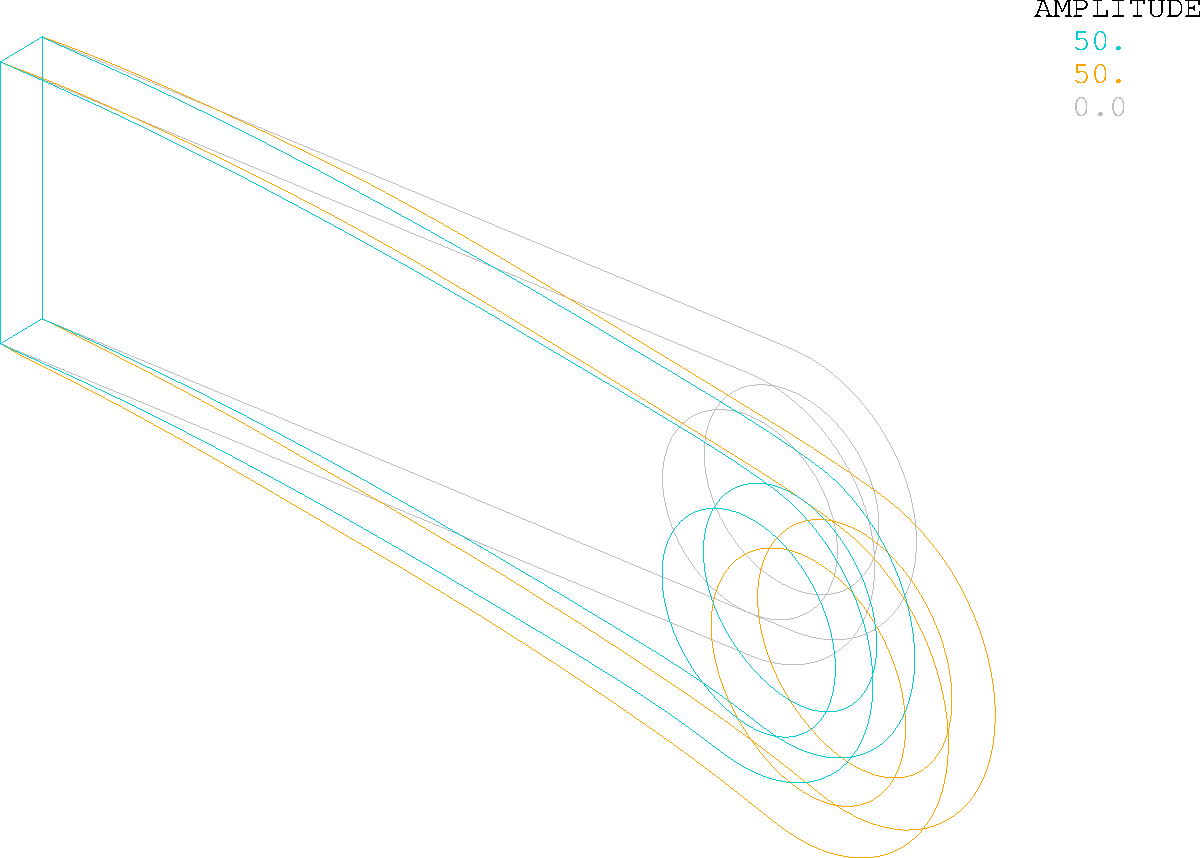
\includegraphics[width=4cm]{images/exo/7_deformee}
    \end{textblock*}
    \onslide<2->{
      \lstinputlisting[language=gibiane, firstline=254, lastline=257]{dgibi/formation_debutant_3_mecanique.dgibi}
      \lstinputlisting[language=gibiane, firstline=262, lastline=262]{dgibi/formation_debutant_3_mecanique.dgibi}
      \begin{textblock*}{5cm}(7.2cm,-2.5cm)
        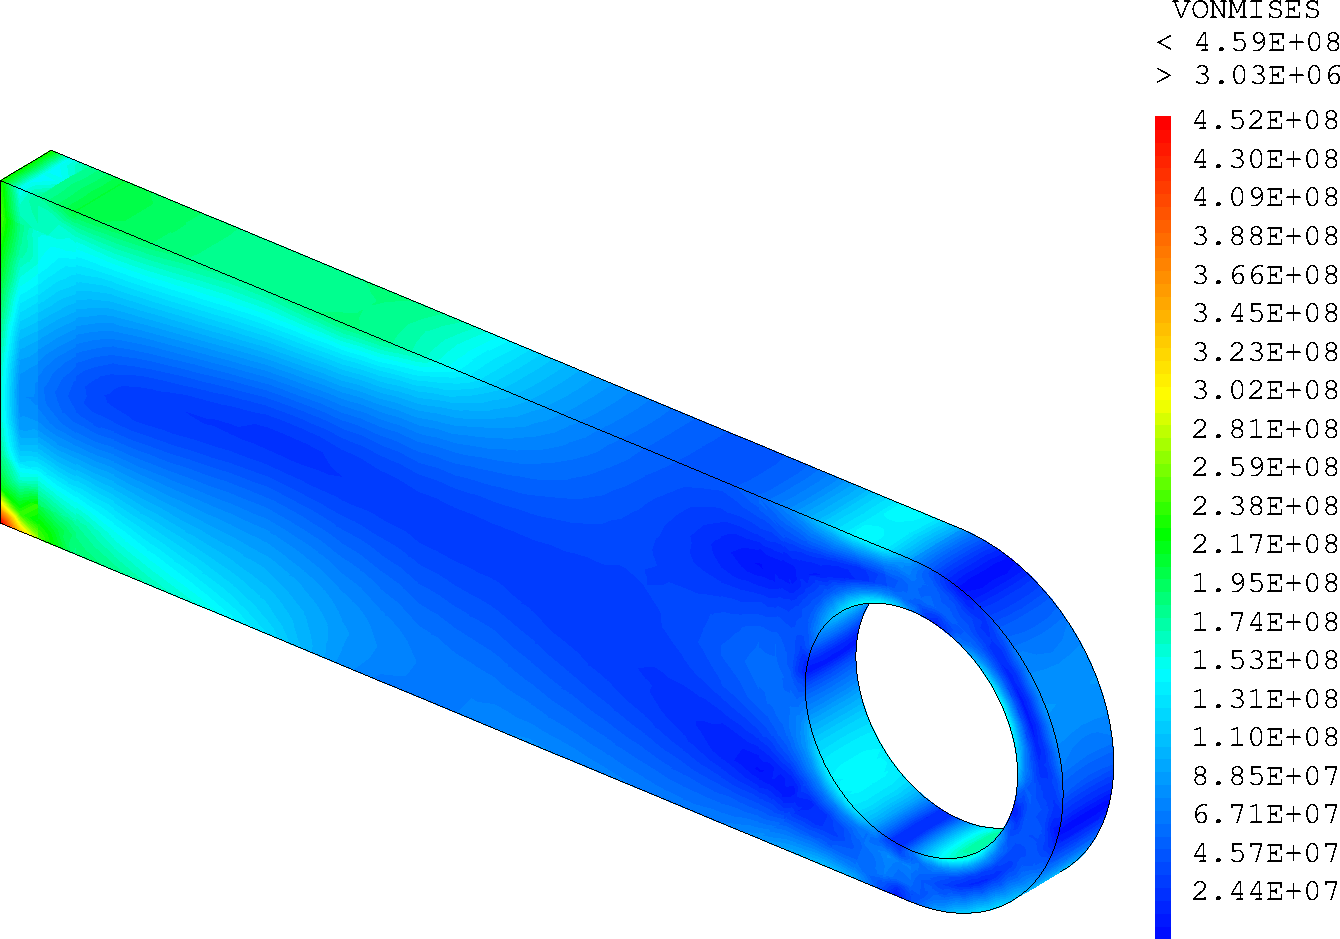
\includegraphics[width=5cm]{images/exo/7_contraintes.pdf}
      \end{textblock*}}
  \end{itemize}
\end{frame}

\begin{frame}{\fe{8 Problème étudié}{8 Problem description}}
  \begin{itemize}
    \item \gray{\fe{Élasticité linéaire}{Linear elasticity}}
    \begin{columns}
      \begin{column}{.4\textwidth}
        \item \gray{\fe{Déplacements imposés}{Imposed displacements}}
        \footnotesize
        \begin{tikzpicture}
          \node[anchor=south west,inner sep=0,opacity=0.3] (image) at (0,0)
          {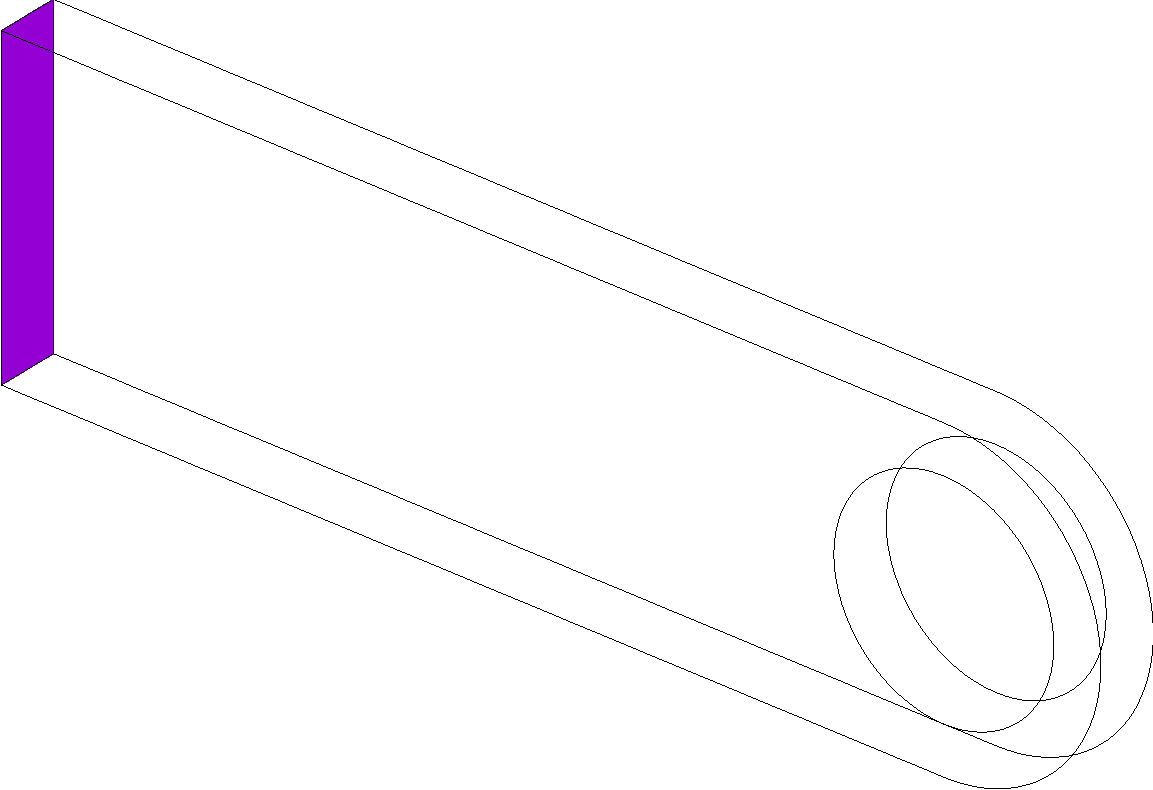
\includegraphics[width=3.5cm]{images/exo/6_cl_deplacement}};
          \begin{scope}[x={(image.south east)},y={(image.north west)},color=violet,opacity=0.3]
            \draw (0.06,0.7) node[anchor=north west] {$u_x=u_y=u_z$~=~0~m};
          \end{scope}
        \end{tikzpicture}
        \normalsize
      \end{column}
      \begin{column}{.4\textwidth}
        \item \gray{\fe{Forces imposées}{Imposed forces}}
        \footnotesize
        \begin{tikzpicture}
          \node[anchor=south west,inner sep=0,opacity=0.3] (image) at (0,0)
          {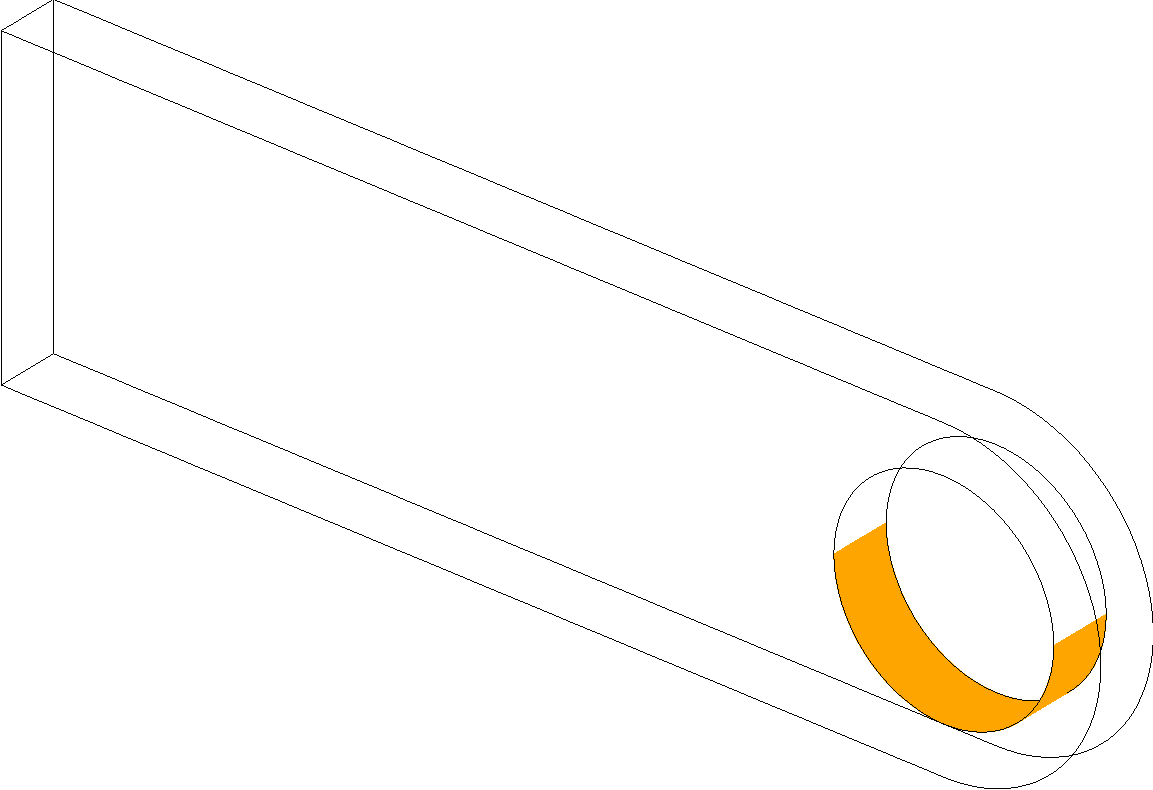
\includegraphics[width=3.5cm]{images/exo/6_cl_force}};
          \begin{scope}[x={(image.south east)},y={(image.north west)},color=orange,opacity=0.3]
            \draw (0.8,0.75) node[anchor=north west] {\fe{masse suspendue}{hanging mass}};
            \draw (0.9,0.6) node[anchor=north west] {$m$~=~2500~kg};
          \end{scope}
        \end{tikzpicture}
        \normalsize
      \end{column}
    \end{columns}
    \begin{columns}
      \begin{column}{.4\textwidth}
        \item \fe{Chargement thermique}{Thermal load}
        \footnotesize
        \begin{tikzpicture}
          \node[anchor=south west,inner sep=0] (image) at (0,0)
          {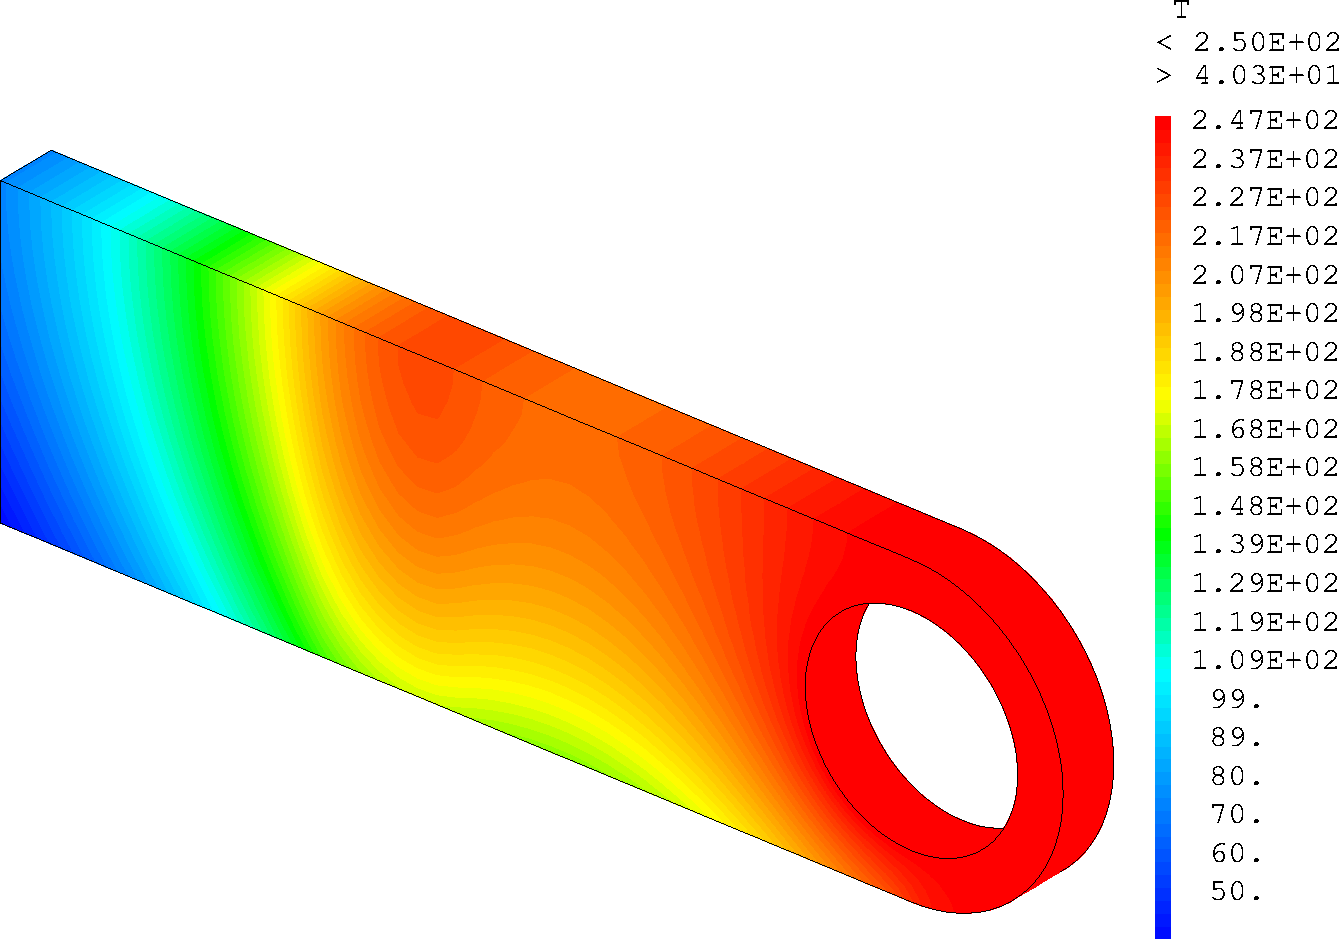
\includegraphics[width=4cm]{images/exo/2.2_temperatures}};
          \begin{scope}[x={(image.south east)},y={(image.north west)},color=blue]
            \draw (0.1,0.2) node {dilatation};
            \draw (0.1,0.05) node {\fe{$\alpha$ \tou{hétérogène}}{$\alpha$ \tou{heterogeneous}}};
          \end{scope}
        \end{tikzpicture}
        \normalsize
      \end{column}
      \begin{column}{.4\textwidth}
      \end{column}
    \end{columns}
  \end{itemize}
\end{frame}

\begin{frame}{\fe{8 Mécanique linéaire}{8 Linear mechanics}}
             {\fe{Élasticité, chargement thermique, matériau hétérogène}
                 {Elasticity, thermal load, heterogeneous matrial}}
  \begin{itemize}
    \item \fe{Coefficient de dilatation $\alpha$ dépendant de $x$ (loi normale)}
             {Thermal expansion coefficient $\alpha$ dependent on $x$ (normal distribution)}
    \footnotesize
    \begin{equation*}
      \alpha(x)=\alpha_0\left(1+3e^{-\left(\frac{x-\mu}{\sigma}\right)^2}\right)
    \end{equation*}
    \footnotesize
    \fe{avec :}{with}
    \begin{itemize}
        \footnotesize
        \item[] $\mu=\frac{l}{2}$ \fe{moyenne}{mean value}
      \item[] $\sigma=\frac{l}{5}$ \fe{écart type}{standard deviation}
    \end{itemize}
    \normalsize
    \onslide<2->{
      \lstinputlisting[language=gibiane, firstline=281, lastline=287]{dgibi/formation_debutant_3_mecanique.dgibi}}
      \onslide<3->{
        \lstinputlisting[language=gibiane, firstline=292, lastline=292]{dgibi/formation_debutant_3_mecanique.dgibi}
        \begin{textblock*}{5cm}(7.2cm,-4.6cm)
          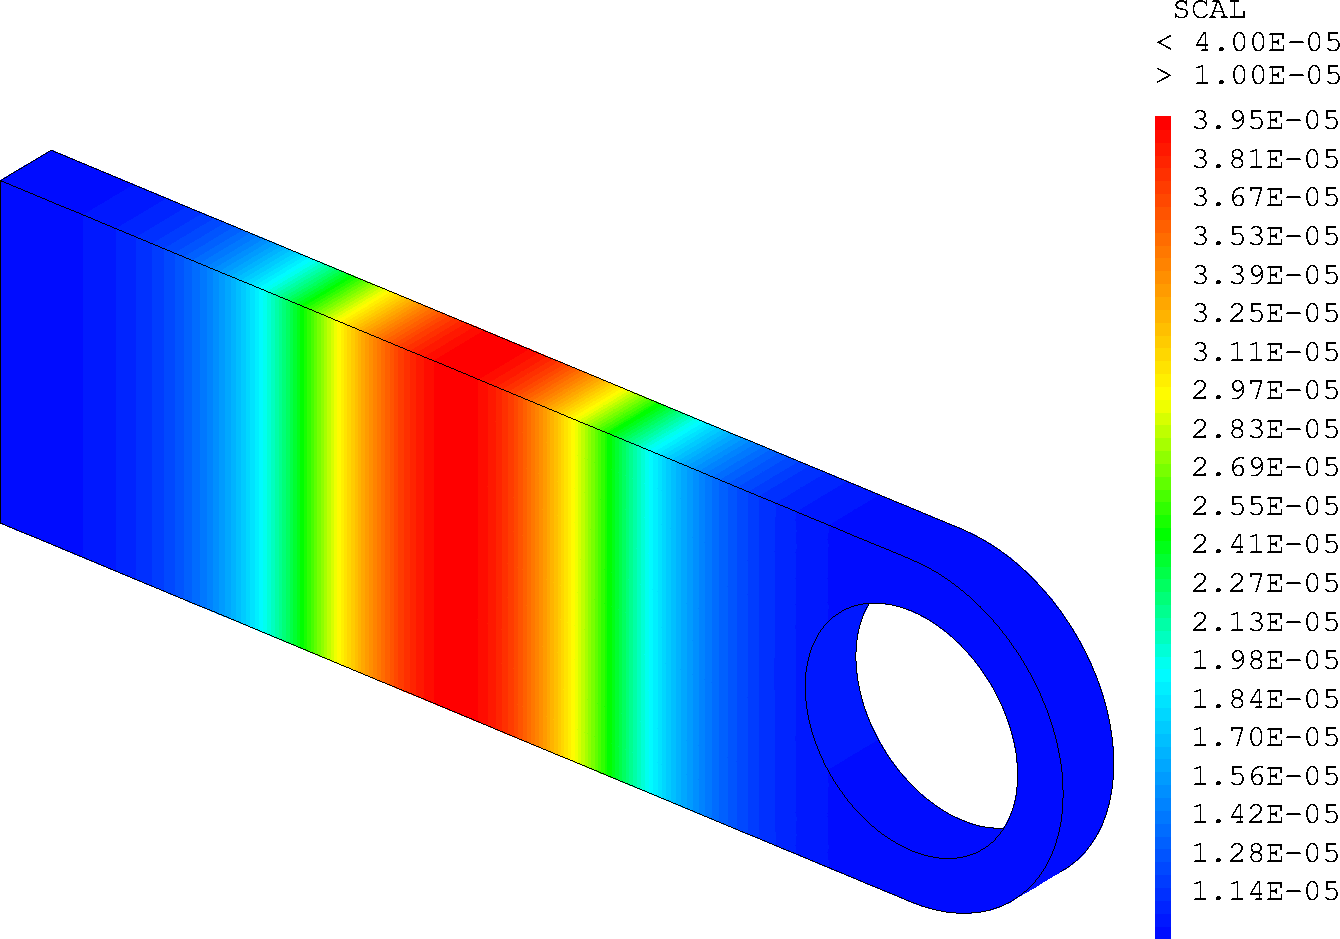
\includegraphics[width=5cm]{images/exo/8_alpha_variable}
        \end{textblock*}}
    \end{itemize}
\end{frame}

\begin{frame}{\fe{8 Mécanique linéaire}{8 Linear mechanics}}
             {\fe{Élasticité, chargement thermique, matériau hétérogène}
                 {Elasticity, thermal load, heterogeneous matrial}}
  \begin{itemize}
    \item \fe{Mise à jour des caractéristiques matériau}
             {Updating the material properties}
    \lstinputlisting[language=gibiane, firstline=294, lastline=299]{dgibi/formation_debutant_3_mecanique.dgibi}
    \item<2->\fe{Mise à jour du chargement thermique}
                {Updating the thermal load}
    \onslide<2->{
        \lstinputlisting[language=gibiane, firstline=301, lastline=304]{dgibi/formation_debutant_3_mecanique.dgibi}}
    \end{itemize}
\end{frame}

\begin{frame}{\fe{8 Mécanique linéaire}{8 Linear mechanics}}
             {\fe{Élasticité, chargement thermique, matériau hétérogène}
                 {Elasticity, thermal load, heterogeneous matrial}}
  \begin{itemize}
    \item \fe{Résolution et affichage des résultats}{Solving and plotting results}
    \lstinputlisting[language=gibiane, firstline=306, lastline=310]{dgibi/formation_debutant_3_mecanique.dgibi}
    \lstinputlisting[language=gibiane, firstline=315, lastline=315]{dgibi/formation_debutant_3_mecanique.dgibi}
    \begin{textblock*}{5cm}(8.2cm,-3.8cm)
      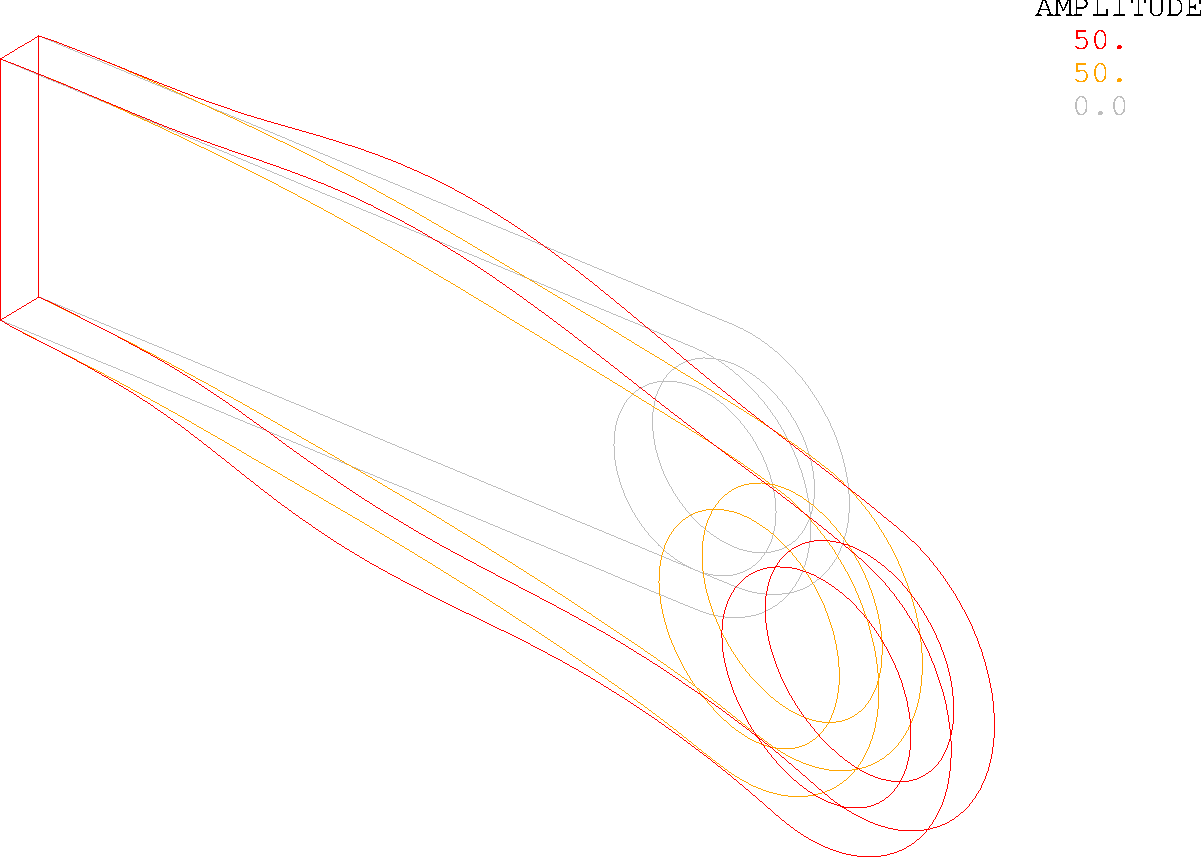
\includegraphics[width=4cm]{images/exo/8_deformee}
    \end{textblock*}
    \onslide<2->{
      \lstinputlisting[language=gibiane, firstline=318, lastline=321]{dgibi/formation_debutant_3_mecanique.dgibi}
      \lstinputlisting[language=gibiane, firstline=326, lastline=326]{dgibi/formation_debutant_3_mecanique.dgibi}
      \begin{textblock*}{5cm}(7.2cm,-2.5cm)
        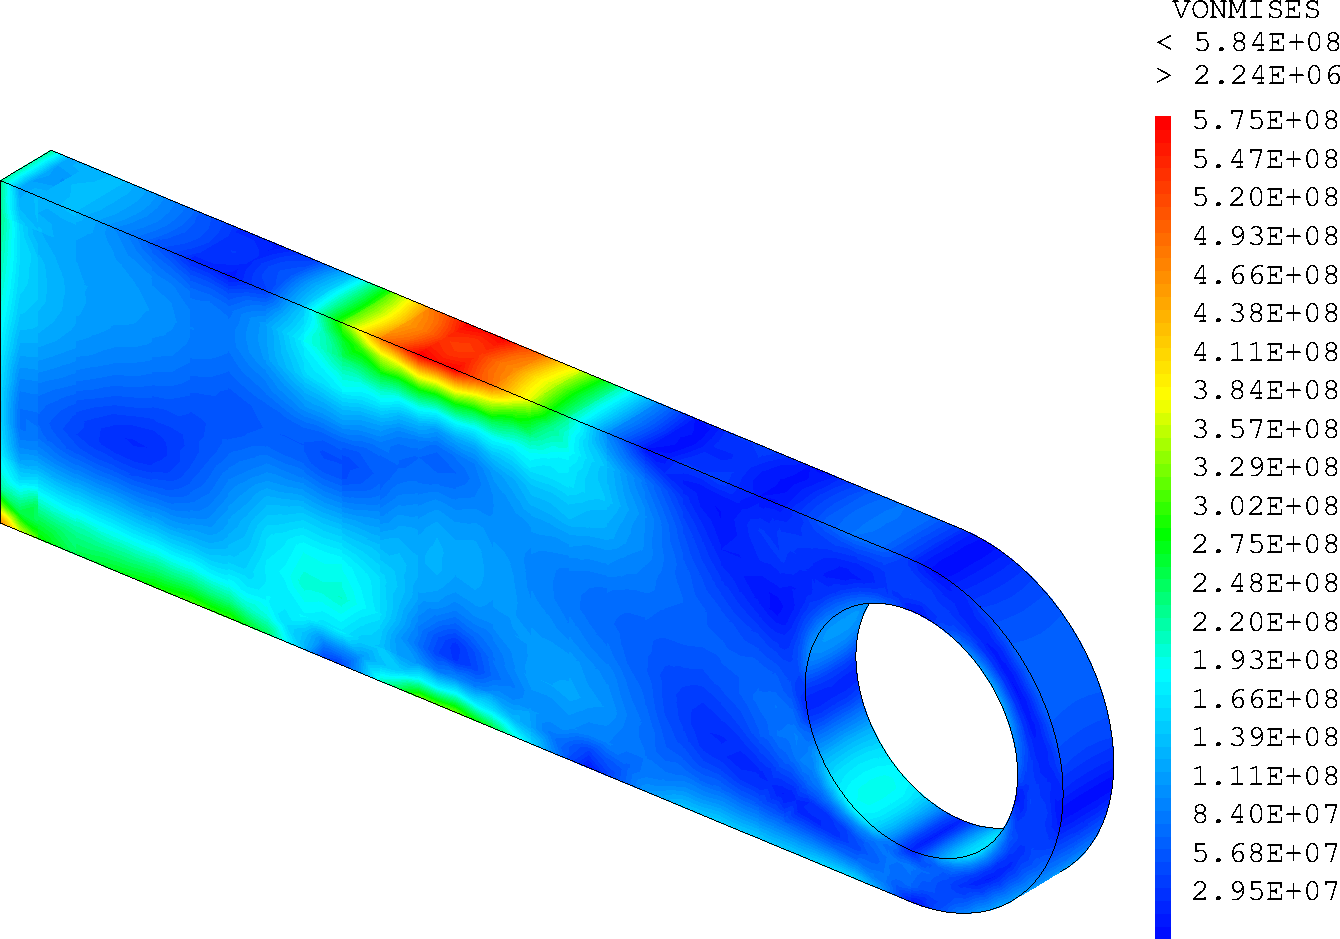
\includegraphics[width=5cm]{images/exo/8_contraintes.pdf}
      \end{textblock*}}
  \end{itemize}
\end{frame}




\fe{\subsection{Thermo mécanique non linéaire}}{\subsection{Non Linear Thermo Mechanics}}
\begin{frame}{\fe{9.1 Problème étudié}{9.1 Problem description}}
  \begin{itemize}
    \item \fe{\tou{Élasto plasticité} (plasticité parfaite)}
             {\tou{Elasto plasticity} (perfect plasticity)}
    \begin{textblock*}{5cm}(8.1cm,-1.8cm)
      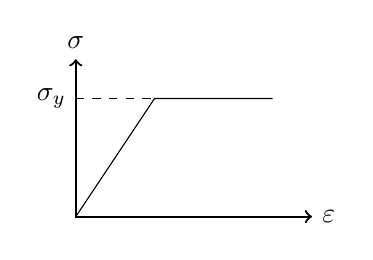
\begin{tikzpicture}
        % axes
        \draw [<->,thick] (0,2) node (yaxis) [above] {$\sigma$}
                       |- (3,0) node (xaxis) [right] {$\varepsilon$};
        % courbe de traction
        \draw (0,0) -- (1,1.5) coordinate (a) -- (2.5,1.5);
        % ligne pour sigy
        \draw[dashed] (yaxis |- a) node[left] {$\sigma_y$} -| (a) ;
      \end{tikzpicture}
    \end{textblock*}
    \begin{center}
    \footnotesize
    \begin{tikzpicture}
      \node[anchor=south west,inner sep=0] (image) at (0,0)
      {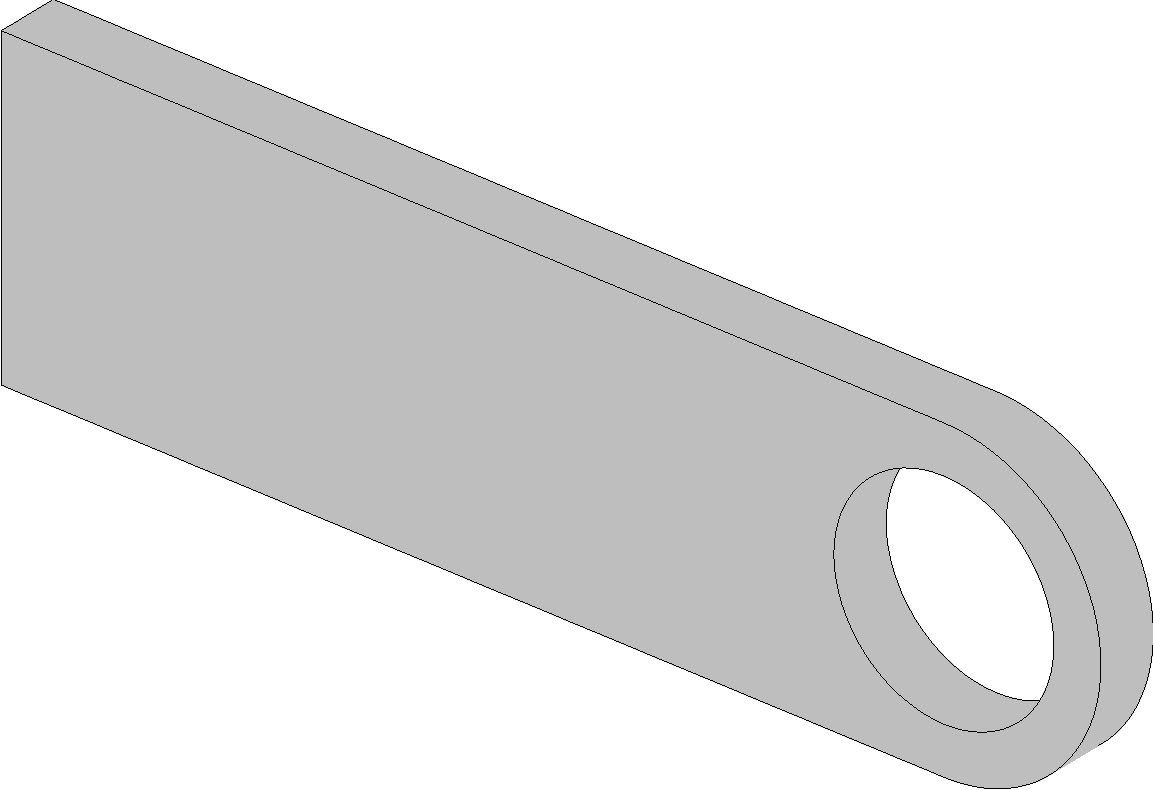
\includegraphics[width=4cm]{images/exo/1.2_geometrie}};
      \begin{scope}[x={(image.south east)},y={(image.north west)}]
        \draw (1,0.9) node[anchor=west] {$E$~=~200~GPa};
        \draw (1,0.7) node[anchor=west] {$\nu$~=~0.3};
        \draw (1,0.5) node[anchor=west] {$\alpha(x)=10^{-5}\left(1+3e^{-\left(\frac{x-\mu}{\sigma}\right)^2}\right)$~K$^{-1}$};
        \draw (1,0.3) node[anchor=west] {\tou{$\sigma_y$~=~250~MPa}};
      \end{scope}
    \end{tikzpicture}
    \normalsize
    \end{center}
    \begin{columns}
      \begin{column}{.4\textwidth}
        \item \gray{\fe{Déplacements imposés}{Imposed displacements}}
      \end{column}
      \begin{column}{.4\textwidth}
        \item \gray{\fe{Forces imposées}{Imposed forces}}
      \end{column}
    \end{columns}
    \begin{columns}
      \begin{column}{.4\textwidth}
        \item \gray{\fe{Chargement thermique}{Thermal load}}
      \end{column}
      \begin{column}{.4\textwidth}
      \end{column}
    \end{columns}
  \end{itemize}
\end{frame}

\begin{frame}{\fe{9.1 Mécanique non linéaire}{9.1 Non linear mechanics}}
             {\fe{Élastoplasticité, chargement thermique, matériau hétérogène}
                 {Elastoplasticity, thermal load, heterogeneous matrial}}
  \begin{itemize}
    \item \fe{Objectif : calcul mécanique \tou{non linéaire} (matériau)}
             {Objective: \tou{non linear} mechanical calculation}
    \begin{equation*}
      \int_{V}[B]^T\{\sigma\}dV=\{F\}
    \end{equation*}
    \item \fe{Méthode :}{Method:}\\
    \begin{tabular}{ll}
      \fe{ajout d'un modèle de plasticité}{adding a plastic model}\\
      \fe{description temporelle des chargements (pseudo temps)}{time description of loads (pseudo time)}\\
      \fe{résolution avec la procédure \kwo{PASAPAS}}{using the \kwo{PASAPAS} solving procedure}\\
    \end{tabular}
  \end{itemize}
\end{frame}

\begin{frame}{\fe{9.1 Mécanique non linéaire}{9.1 Non linear mechanics}}
             {\fe{Élastoplasticité, chargement thermique, matériau hétérogène}
                 {Elastoplasticity, thermal load, heterogeneous matrial}}
  \begin{itemize}
    \item \fe{Formulation mathématique (élasticité)}{Mathematical formulation (elasticity)}
    \lstinputlisting[basicstyle=\ttfamily\tiny, language=gibiane, firstline=46, lastline=46]{dgibi/formation_debutant_3_mecanique.dgibi}
    \lstinputlisting[basicstyle=\ttfamily\tiny, language=gibiane, firstline=345, lastline=349]{dgibi/formation_debutant_3_mecanique.dgibi}
    \item<2->\fe{Chargements : description temporelle}{Loads: time description}
    \lstinputlisting[basicstyle=\ttfamily\tiny, language=gibiane, firstline=353, lastline=355]{dgibi/formation_debutant_3_mecanique.dgibi}
    \lstinputlisting[basicstyle=\ttfamily\tiny, language=gibiane, firstline=356, lastline=363]{dgibi/formation_debutant_3_mecanique.dgibi}
    \end{itemize}
\end{frame}

\begin{frame}{\fe{9.1 Mécanique non linéaire}{9.1 Non linear mechanics}}
             {\fe{Élastoplasticité, chargement thermique, matériau hétérogène}
                 {Elastoplasticity, thermal load, heterogeneous matrial}}
  \begin{itemize}
    \item \fe{Résolution avec \kwo{PASAPAS}}{Solving with \kwo{PASAPAS}}\\
    \avous{\fe{Remplir la TABLE et lancer \kw{PASAPAS}}{Fill the TABLE and launch \kw{PASAPAS}}}
    \onslide<2->{
      \lstinputlisting[language=gibiane, firstline=365, lastline=373]{dgibi/formation_debutant_3_mecanique.dgibi}}
    \end{itemize}
\end{frame}

\begin{frame}{\fe{9.1 Mécanique non linéaire}{9.1 Non linear mechanics}}
             {\fe{Élastoplasticité, chargement thermique, matériau hétérogène}
                 {Elastoplasticity, thermal load, heterogeneous matrial}}
  \begin{itemize}
    \item \fe{Post traitement : boucle de tracés}{Post processing: loop for plot}
    \lstinputlisting[basicstyle=\ttfamily\tiny, language=gibiane, firstline=381, lastline=387]{dgibi/formation_debutant_3_mecanique.dgibi}
    \lstinputlisting[basicstyle=\ttfamily\tiny, language=gibiane, firstline=389, lastline=389]{dgibi/formation_debutant_3_mecanique.dgibi}
    \lstinputlisting[basicstyle=\ttfamily\tiny, language=gibiane, firstline=391, lastline=391]{dgibi/formation_debutant_3_mecanique.dgibi}
  \end{itemize}
  \begin{textblock*}{5cm}(7cm,-1cm)
    \animategraphics[controls,loop,poster=last,width=5cm]{10}{images/exo/9.1_contraintes.}{01}{21}
  \end{textblock*}
  \vspace{3cm}
\end{frame}

\begin{frame}{\fe{9.1 Mécanique non linéaire}{9.1 Non linear mechanics}}
             {\fe{Élastoplasticité, chargement thermique, matériau hétérogène}
                 {Elastoplasticity, thermal load, heterogeneous matrial}}
  \begin{itemize}
    \item \fe{Post traitement : boucle de tracés}{Post processing: loop for plot}
    \lstinputlisting[basicstyle=\ttfamily\tiny, language=gibiane, firstline=398, lastline=404]{dgibi/formation_debutant_3_mecanique.dgibi}
    \lstinputlisting[basicstyle=\ttfamily\tiny, language=gibiane, firstline=406, lastline=406]{dgibi/formation_debutant_3_mecanique.dgibi}
    \lstinputlisting[basicstyle=\ttfamily\tiny, language=gibiane, firstline=408, lastline=408]{dgibi/formation_debutant_3_mecanique.dgibi}
  \end{itemize}
  \begin{textblock*}{5cm}(7cm,-1cm)
    \animategraphics[controls,loop,poster=last,width=5cm]{10}{images/exo/9.1_variables_internes.}{01}{21}
  \end{textblock*}
  \vspace{3cm}
\end{frame}

\begin{frame}{\fe{9.2 Problème étudié}{9.2 Problem description}}
  \begin{itemize}
    \item \fe{Élasto plasticité (plasticité parfaite), \tou{dépendance à la température}}
             {Elasto plasticity (perfect plasticity), \tou{temperature dependent}}
    \begin{center}
    \footnotesize
    \begin{tikzpicture}
      \node[anchor=south west,inner sep=0] (image) at (0,0)
      {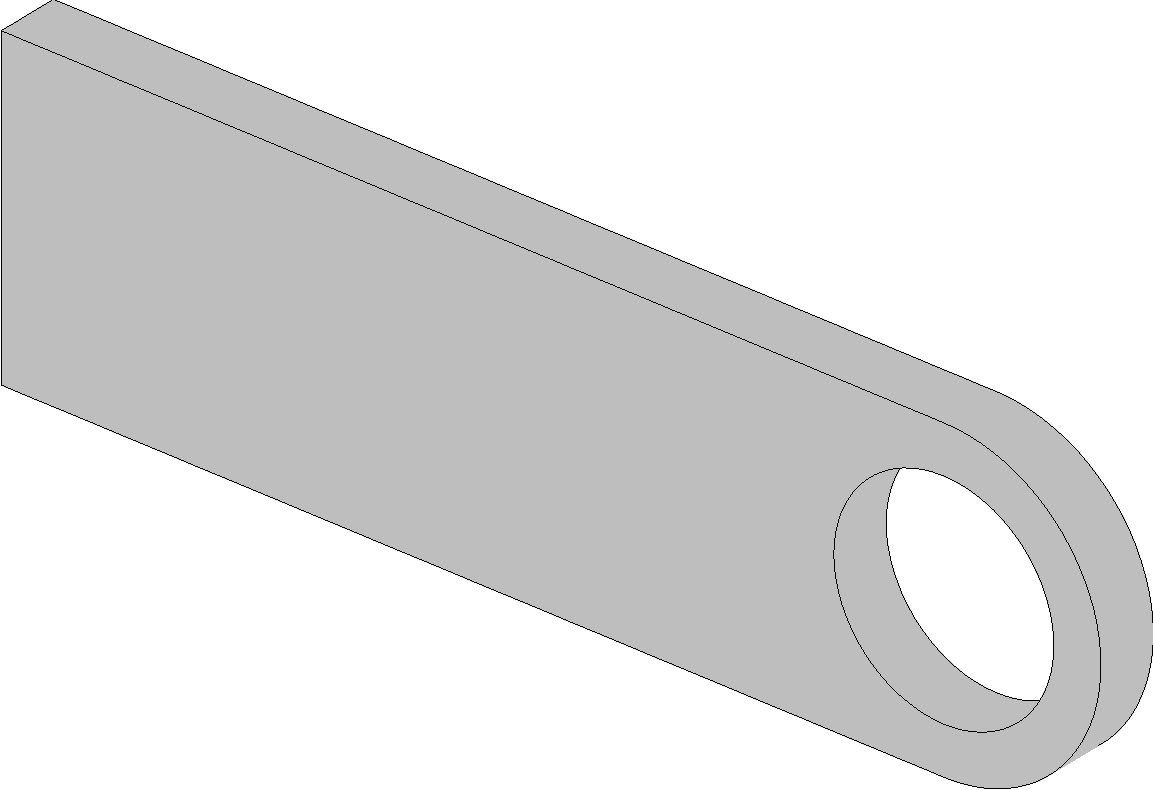
\includegraphics[width=4cm]{images/exo/1.2_geometrie}};
      \begin{scope}[x={(image.south east)},y={(image.north west)}]
        \draw (1,0.9) node[anchor=west] {$E$~=~200~GPa};
        \draw (1,0.7) node[anchor=west] {$\nu$~=~0.3};
        \draw (1,0.5) node[anchor=west] {$\alpha(x)=10^{-5}\left(1+3e^{-\left(\frac{x-\mu}{\sigma}\right)^2}\right)$~K$^{-1}$};
        \draw (1,0.3) node[anchor=west] {\tou{$\sigma_y=f(T)$}};
      \end{scope}
    \end{tikzpicture}
    \normalsize
    \end{center}
    \begin{columns}
      \begin{column}{.4\textwidth}
        \item \gray{\fe{Déplacements imposés}{Imposed displacements}}
      \end{column}
      \begin{column}{.4\textwidth}
        \item \gray{\fe{Forces imposées}{Imposed forces}}
      \end{column}
    \end{columns}
    \begin{columns}
      \begin{column}{.4\textwidth}
        \item \gray{\fe{Chargement thermique}{Thermal load}}
      \end{column}
      \begin{column}{.4\textwidth}
      \end{column}
    \end{columns}
  \end{itemize}
\end{frame}

\begin{frame}{\fe{9.2 Mécanique non linéaire}{9.2 Non linear mechanics}}
             {\fe{Élastoplasticité, chargement thermique, matériau hétérogène, T dépendant}
                 {Elastoplasticity, thermal load, heterogeneous matrial, T dependent}}
  \begin{itemize}
    \item \fe{Dépendance d'un paramètre à la température}{Temperature dependence of a parameter}
    \lstinputlisting[basicstyle=\ttfamily\tiny, language=gibiane, firstline=428, lastline=432]{dgibi/formation_debutant_3_mecanique.dgibi}
    \onslide<2->{
      \lstinputlisting[basicstyle=\ttfamily\tiny, language=gibiane, firstline=437, lastline=437]{dgibi/formation_debutant_3_mecanique.dgibi}
      \begin{textblock*}{5cm}(8.1cm,0cm)
        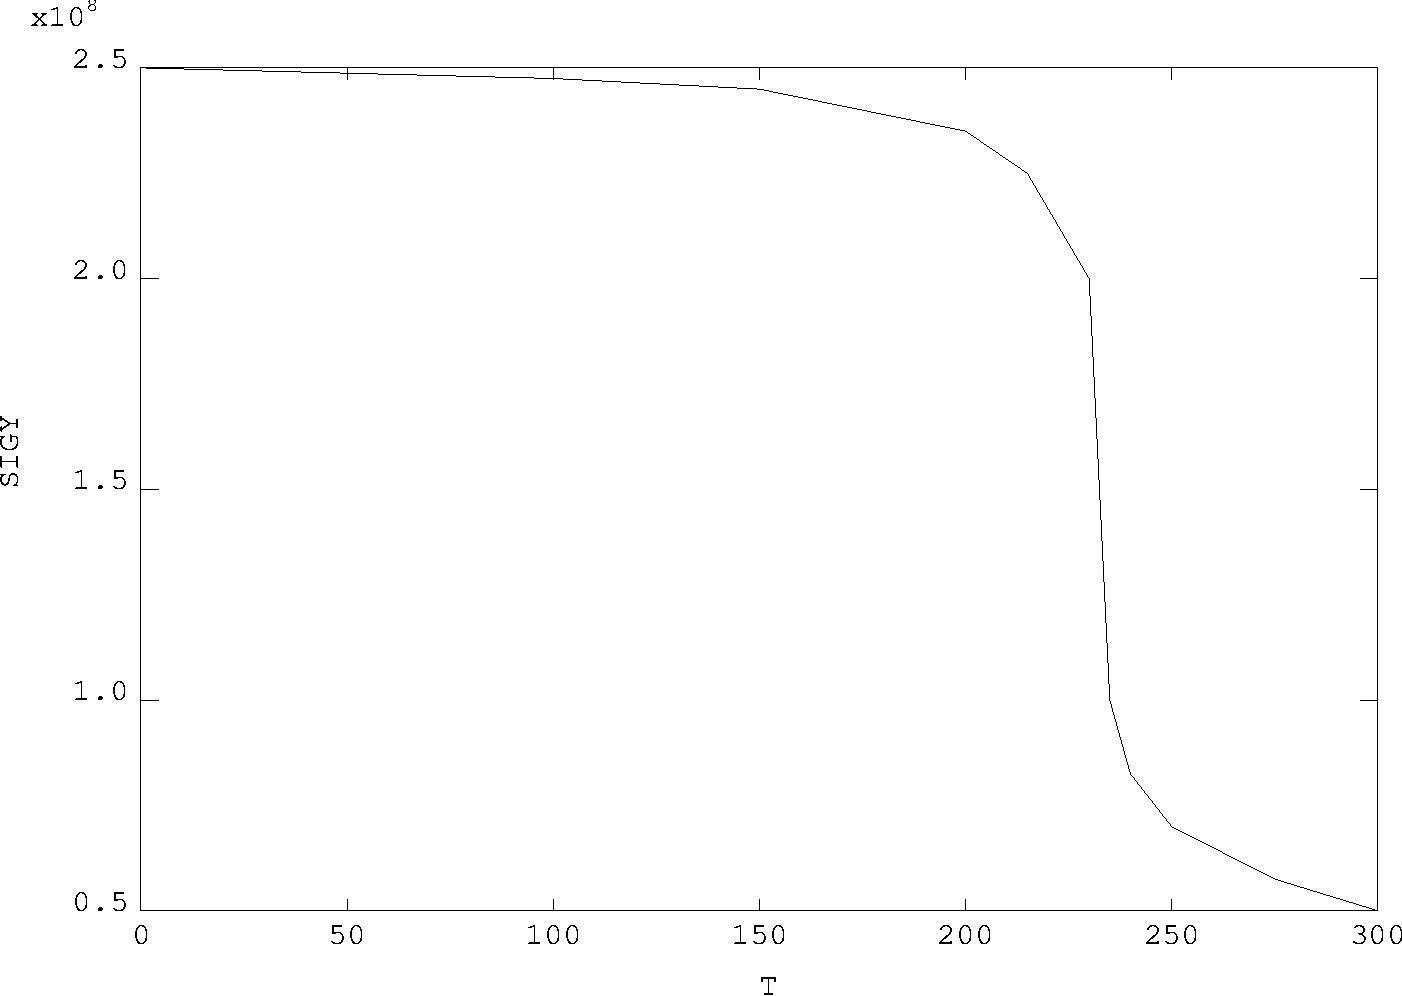
\includegraphics[width=4.3cm]{images/exo/9.2_evol_sigy}
      \end{textblock*}}
    \item<3->\fe{Mise à jour des caractéristiques matériau}{Updating the material properties}
    \onslide<3->{
      \lstinputlisting[basicstyle=\ttfamily\tiny, language=gibiane, firstline=440, lastline=443]{dgibi/formation_debutant_3_mecanique.dgibi}}
  \end{itemize}
\end{frame}

\begin{frame}{\fe{9.2 Mécanique non linéaire}{9.2 Non linear mechanics}}
             {\fe{Élastoplasticité, chargement thermique, matériau hétérogène, T dépendant}
                 {Elastoplasticity, thermal load, heterogeneous matrial, T dependent}}
  \begin{itemize}
    \item \fe{Résolution avec \kwo{PASAPAS}}{Solving with \kwo{PASAPAS}}
    \lstinputlisting[language=gibiane, firstline=445, lastline=453]{dgibi/formation_debutant_3_mecanique.dgibi}
  \end{itemize}
\end{frame}

\begin{frame}{\fe{9.2 Mécanique non linéaire}{9.2 Non linear mechanics}}
             {\fe{Élastoplasticité, chargement thermique, matériau hétérogène, T dépendant}
                 {Elastoplasticity, thermal load, heterogeneous matrial, T dependent}}
  \begin{itemize}
    \item \fe{Post traitement : boucle de tracés}{Post processing: loop for plot}
    \lstinputlisting[basicstyle=\ttfamily\tiny, language=gibiane, firstline=456, lastline=456]{dgibi/formation_debutant_3_mecanique.dgibi}
    \lstinputlisting[basicstyle=\ttfamily\tiny, language=gibiane, firstline=462, lastline=468]{dgibi/formation_debutant_3_mecanique.dgibi}
    \lstinputlisting[basicstyle=\ttfamily\tiny, language=gibiane, firstline=470, lastline=470]{dgibi/formation_debutant_3_mecanique.dgibi}
    \lstinputlisting[basicstyle=\ttfamily\tiny, language=gibiane, firstline=472, lastline=472]{dgibi/formation_debutant_3_mecanique.dgibi}
    \lstinputlisting[basicstyle=\ttfamily\tiny, language=gibiane, firstline=476, lastline=476]{dgibi/formation_debutant_3_mecanique.dgibi}
  \end{itemize}
  \begin{textblock*}{5cm}(7cm,-1.4cm)
    \animategraphics[controls,loop,poster=last,width=5cm]{10}{images/exo/9.2_variables_internes.}{01}{21}
  \end{textblock*}
  \vspace{3cm}
\end{frame}
